%input macros (i.e. write your own macros file called MacroFile1.tex)
%\newcommand{\PdfPsText}[2]{
  \ifpdf
     #1
  \else
     #2
  \fi
}

\newcommand{\IncludeGraphicsH}[3]{
  \PdfPsText{\includegraphics[height=#2]{#1}}{\includegraphics[bb = #3, height=#2]{#1}}
}

\newcommand{\IncludeGraphicsW}[3]{
  \PdfPsText{\includegraphics[width=#2]{#1}}{\includegraphics[bb = #3, width=#2]{#1}}
}

\newcommand{\InsertFig}[3]{
  \begin{figure}[!htbp]
    \begin{center}
      \leavevmode
      #1
      \caption{#2}
      \label{#3}
    \end{center}
  \end{figure}
}


%%% Local Variables: 
%%% mode: latex
%%% TeX-master: "~/Documents/LaTeX/CUEDThesisPSnPDF/thesis"
%%% End: 



\documentclass[oneside,12pt]{Classes/IITRPRBTP}

\ifpdf
    \pdfinfo { /Title  (IIT Ropar BTech Project Report Classes)
               /Creator (TeX)
               /Producer (pdfTeX)
               /Author (Jagpreet Singh jagpreets@iitrpr.ac.in)
               /CreationDate (D:20120326000000)  %format D:YYYYMMDDhhmmss
               /ModDate (D:20120326000000)
               /Subject (Writing a BTech Project Report in LaTeX)
               /Keywords (BTP)}
    \pdfcatalog { /PageMode (/UseOutlines)
                  /OpenAction (fitbh)  }
\fi

\title{MRI enhancements using neural networks}

\renewcommand{\submittedtext}{A Project Report Submitted \\ in Partial Fulfillment of Requirements \\ for the Degree of}
\degree{Bachelor of Technology}
\degreedate{May 2023}

\ifpdf
  \author{\href{mailto:2019csb1064@iitrpr.ac.in}{by} \\ {Aditya Agarwal(2019CSB1064)} \\ \href{mailto:2019csb1119@iitrpr.ac.in}{Shikhar Soni (2019CSB1119)}}
  \collegeordept{\href{http://www.iitrpr.ac.in}{Department of Computer Science \& Engineering }}
  \university{\href{http://www.iitrpr.ac.in}{Indian Institute of Technology Ropar}}
  \city{{Rupnagar 140001, Punjab, India}}
% insert below the file name that contains the crest in-place of 'IITRPRlogo'
  \crest{
\includegraphics[width=20mm]{IITRPRlogo}}
%\else
%  \author{Jagpreet Singh}
%  \collegeordept{Department of Computer Science \& Engineering}
%  \university{Indian Institute of Technology Ropar}
% insert below the file name that contains the crest in-place of 'IITRPRlogo'
%  \crest{
\includegraphics[bb = 0 0 292 336, width=30mm]{IITRPRlogo}}
\fi
%
% insert below the file name that contains the crest in-place of 'IITRPRlogo'
% \crest{\IncludeGraphicsW{IITRPRlogo}{40mm}{14 14 73 81}}
%

% turn of those nasty overfull and underfull hboxes
\hbadness=10000
\hfuzz=50pt

% Put all the style files you want in the directory StyleFiles and usepackage like this:
%\usepackage{StyleFiles/watermark}

% Comment out the next line to get single spacing
\onehalfspacing
\usepackage{array}

\begin{document}

%\language{english}

% A page with the abstract on including title and author etc may be
% required to be handed in separately. If this is not so, then comment
% the below 3 lines (between '\begin{abstractseparte}' and 
% 'end{abstractseparate}'), normally like a declaration ... needs some more
% work, mind as environment abstracts creates a new page!
% \begin{abstractseparate}
%   
% Thesis Abstract -----------------------------------------------------


% \begin{abstractslong}    %uncommenting this line, gives a different abstract heading
\begin{abstracts}        %this creates the heading for the abstract page

Magnetic Resonance Imaging (MRI) is an essential medical imaging technique for diagnosing and monitoring various diseases. However, the low signal-to-noise ratio and long acquisition times of MR images can limit their clinical utility. In recent years, deep learning-based techniques have been proposed to enhance MR images.

In this project, we mainly explore two different methods to enhance MR images, one includes the use of U-Nets to obtain a close to fully sampled MRI from under-sampled MRI and the other includes the use of diffusion models to convert a low-resolution MRI to a higher resolution.

The first proposed approach is for getting a fully sampled MRI image from an under-sampled one. Here we train two U-Net models joined together to form a W-Net model, the input of the model is 3 consecutive slices of an MRI and it uses locality to improve on the previously existing W-net architecture \cite{8919674}.

The second proposed approach for getting a higher resolution image from a lower resolution one works by using diffusion models and tries to improve on the known Super Resolution (SR) models \cite{saharia2021image} to get good results for MRIs while ensuring minimum artefacts.

In conclusion, our study highlights the potential of deep learning-based approaches for enhancing MR images and provides insights into the benefits of using diffusion models and combined U-Net models (W-Net with locality) in this context.

\end{abstracts}
% \end{abstractslong}


% ----------------------------------------------------------------------


%%% Local Variables: 
%%% mode: latex
%%% TeX-master: "../thesis"
%%% End: 

% \end{abstractseparate}

% Using the watermark package which is in StyleFiles/
% and to remove DRAFT COPY ONLY appearing on the top of all pages comment out below line
%\watermark{DRAFT COPY ONLY}

\maketitle

%set the number of sectioning levels that get number and appear in the contents
\setcounter{secnumdepth}{3}
\setcounter{tocdepth}{3}

\frontmatter % book mode only
\pagenumbering{roman}
%% Thesis Dedictation ---------------------------------------------------

\begin{dedication} %this creates the heading for the dedication page

I would like to dedicate this thesis to my loving parents ...

\end{dedication}

% ----------------------------------------------------------------------

%%% Local Variables: 
%%% mode: latex
%%% TeX-master: "../thesis"
%%% End: 


% Thesis Abstract -----------------------------------------------------


% \begin{abstractslong}    %uncommenting this line, gives a different abstract heading
\begin{abstracts}        %this creates the heading for the abstract page

Magnetic Resonance Imaging (MRI) is an essential medical imaging technique for diagnosing and monitoring various diseases. However, the low signal-to-noise ratio and long acquisition times of MR images can limit their clinical utility. In recent years, deep learning-based techniques have been proposed to enhance MR images.

In this project, we mainly explore two different methods to enhance MR images, one includes the use of U-Nets to obtain a close to fully sampled MRI from under-sampled MRI and the other includes the use of diffusion models to convert a low-resolution MRI to a higher resolution.

The first proposed approach is for getting a fully sampled MRI image from an under-sampled one. Here we train two U-Net models joined together to form a W-Net model, the input of the model is 3 consecutive slices of an MRI and it uses locality to improve on the previously existing W-net architecture \cite{8919674}.

The second proposed approach for getting a higher resolution image from a lower resolution one works by using diffusion models and tries to improve on the known Super Resolution (SR) models \cite{saharia2021image} to get good results for MRIs while ensuring minimum artefacts.

In conclusion, our study highlights the potential of deep learning-based approaches for enhancing MR images and provides insights into the benefits of using diffusion models and combined U-Net models (W-Net with locality) in this context.

\end{abstracts}
% \end{abstractslong}


% ----------------------------------------------------------------------


%%% Local Variables: 
%%% mode: latex
%%% TeX-master: "../thesis"
%%% End: 

% Thesis Acknowledgements ------------------------------------------------


\begin{acknowledgementslong} %uncommenting this line, gives a different acknowledgements heading
% \begin{acknowledgements}      %this creates the heading for the acknowlegments


We would like to express our sincere gratitude to our project mentor, Dr Deepti R. Bathula, for her invaluable guidance and support throughout the course of this project. Her expertise in the field of MRI enhancement and her willingness to share her knowledge has been instrumental in the success of this project. Her constant feedback and encouragement helped us to stay motivated and focused.\\

We would also like to thank our faculty advisor, Dr T.V. Kalyan, for his support and guidance in conducting this project course. His knowledge and experience in the field of computer science have been invaluable in shaping our approach to this project.\\

We also want to extend our heartfelt gratitude to Dr Puneet Goyal and Dr Abhinav Dhall, who evaluated our project and provided valuable feedback. Their insights and suggestions helped us to improve our project and make it more robust.\\

Finally, we thank all the staff members of our department who provided us with the necessary facilities and resources to conduct this project. Mr Ashu Kaushik has been helpful in providing us with the resources necessary for the completion of this project and helped sort out any technical issues.


% \end{acknowledgements}
\end{acknowledgementslong}

% ------------------------------------------------------------------------

%%% Local Variables: 
%%% mode: latex
%%% TeX-master: "../thesis"
%%% End: 

% Project Owner Code ------------------------------------------------



\begin{honorcode}      %this creates the heading for the certificate

We certify that we have properly cited any material taken from other sources and have obtained permission for any
copyrighted material included in this report. We take full responsibility for any code submitted as part of this 
project and the contents of this report. \\

\vspace*{20mm}

\begin{flushright}
Aditya Agarwal ( 2019CSB1064 ) \\ \vspace*{20mm} Shikhar Soni ( 2019CSB1119 ) \\ 
\end{flushright}

\end{honorcode}


% ------------------------------------------------------------------------

%%% Local Variables: 
%%% mode: latex
%%% TeX-master: "../thesis"
%%% End: 

% Project Certificate ------------------------------------------------



\begin{certificate}      %this creates the heading for the certificate

It is certified that the B. Tech. project ``MRI Enhancements using Neural Networks" has been done by Aditya Agarwal (2019CSB1064), Shikhar Soni (2019CSB1119) under my supervision. 
This report has been submitted towards partial fulfillment of B. Tech. project requirements. \\

\vspace*{20mm}

\begin{flushright}
Dr. Deepti R. Bathula \\ Project Supervisor \\ Department of Computer Science \& Engineering \\ Indian Institute of Technology Ropar \\ Rupnagar-140001
\end{flushright}


\end{certificate}


% ------------------------------------------------------------------------

%%% Local Variables: 
%%% mode: latex
%%% TeX-master: "../thesis"
%%% End: 


\tableofcontents

\listoffigures
\listoftables
\printnomenclature  %% Print the nomenclature
\addcontentsline{toc}{chapter}{Nomenclature}

\mainmatter % book mode only
%%% Thesis Introduction --------------------------------------------------
\chapter{Introduction}
\ifpdf
    \graphicspath{{Introduction/IntroductionFigs/PNG/}{Introduction/IntroductionFigs/PDF/}{Introduction/IntroductionFigs/}}
\else
    \graphicspath{{Introduction/IntroductionFigs/EPS/}{Introduction/IntroductionFigs/}}
\fi

Medical imaging has become a crucial tool in the diagnosis and treatment of various diseases, and the development of new image-processing techniques can help improve the quality and speed of medical imaging, especially MRIs.\\

\nomenclature[zmri]{$MRI$}{Magnetic Resonance Imaging}

Our report is mostly concerned with the use of MRIs, they use magnetic fields and radio waves to create detailed images of the inside of the body, especially useful for soft tissues such as the brain, muscles, and organs. MRIs are non-invasive and do not use ionizing radiation, making them a safer alternative to other imaging technologies such as X-rays or CT scans. However, MRIs can also be expensive and time-consuming to perform, and some patients may not be able to tolerate the confined space of the MRI machine.\\

\begin{figure}[!htbp]
  \begin{center}
    \leavevmode
    \ifpdf
      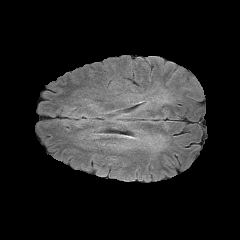
\includegraphics[height=3in]{Introduction/IntroductionFigs/volume_2_slice_88.png}
    \else
      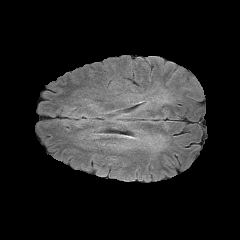
\includegraphics[bb = 92 86 545 742, height=6in]{Introduction/IntroductionFigs/volume_2_slice_88.png}
    \fi
    \caption{A Brain MRI slice \cite{menze2015multimodal, bakas2017advancing, bakas2018identifying}}
    \label{RandomMRI}
  \end{center}
\end{figure}

In recent years, there has been an increased interest in using neural networks to help with this process. We propose two solutions to tackle two of the most important problems concerning MRI.\\

The first problem involves speeding up the process of taking an MRI. To speed up an MRI, we must be able to use the under-sampled MRI that takes lesser time to construct than a fully-sampled MRI output i.e, MRI Reconstruction problem (Section \ref{sec:prob_1} discusses the problem in more detail). Our solution to this problem involves the use of the pre-existing W-Net architecture~\cite{8919674}. The W-Net architecture involves the use of two U-Nets joined together in such a way that the output of one is supplied to the other as input. The first residual U-Net works with the k-space domain MRI data and the second residual U-Net works with the image domain MRI data.\\

Our improvement to this model works with the following idea in mind -- neighbouring MRI slices show very little variations between each other. In our approach, we take only 3 neighbouring slices to show any improvements. The model now takes 3 slices as input and outputs a single close-to-fully-sampled MR image for the middle slice. The neighbours help in providing local information relevant to constructing the middle slice's fully sampled version.\\

The next problem being explored is the well-known problem of super-resolution in MRIs (Section \ref{sec:prob_2} discusses the problem in more detail). In MRIs, however, it's harder to perform super-resolution because we have to ensure that there are minimal artefacts introduced during the super-resolution process. Our approach to solving this problem involves the use of the pre-existing SR3 network \cite{saharia2021image}. Here we don't use MSE (Mean Square Error) as a judgement parameter for the likeness of two images because it doesn't ensure minimisation of artefacts, instead, we propose the use of SSIM (Structural Similarity Index) \cite{1284395} and FID (Fréchet Inception Distance) \cite{fid, mathiasen2021backpropagating}  as both of them promote higher structural similarity. We also want to minimize the noise in the model, a common occurrence in the result of diffusion models such as SR3, so we must also give some weightage to MSE as well.\\

\nomenclature[zssim]{$SSIM$}{Structural Similarity Index}
\nomenclature[zfid]{$FID$}{Fréchet Inception Distance}

Keeping the above in mind, we experimented with variations of the above to study the best use case for MRIs. Our report covers how the difference impacts MRI quality and tries to study the introduction of artefacts.\\

In the report, we aim to show the usefulness of both solutions and how they stand against their baseline counterparts.

%%% ----------------------------------------------------------------------


%%% Local Variables: 
%%% mode: latex
%%% TeX-master: "../thesis"
%%% End: 

% \pagebreak[4]
% \hspace*{1cm}
% \pagebreak[4]
% \hspace*{1cm}
% \pagebreak[4]

\chapter{Existing solutions for the problem space}
\ifpdf
    \graphicspath{{Chapter1/Chapter1Figs/PNG/}{Chapter1/Chapter1Figs/PDF/}{Chapter1/Chapter1Figs/}}
\else
    \graphicspath{{Chapter1/Chapter1Figs/EPS/}{Chapter1/Chapter1Figs/}}
\fi

\nomenclature[zEDSR]{$EDSR$}{Enhanced Deep Super-Resolution Network}
\nomenclature[zPSNR]{$PSNR$}{Peak Signal-to-Noise Ratio}

\section{Enhanced Deep Super-Resolution Network (EDSR)}

\begin{figure}[!htbp]
  \begin{center}
    \leavevmode
    \ifpdf
      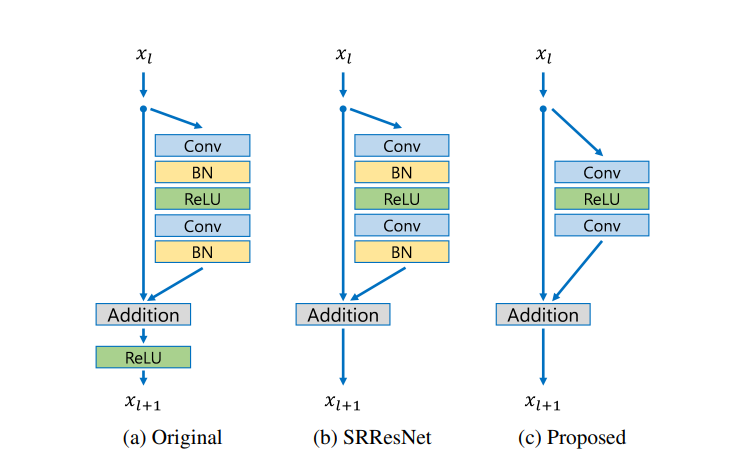
\includegraphics[height=3in]{Chapter1/Chapter1Figs/edsr.png}
    \else
      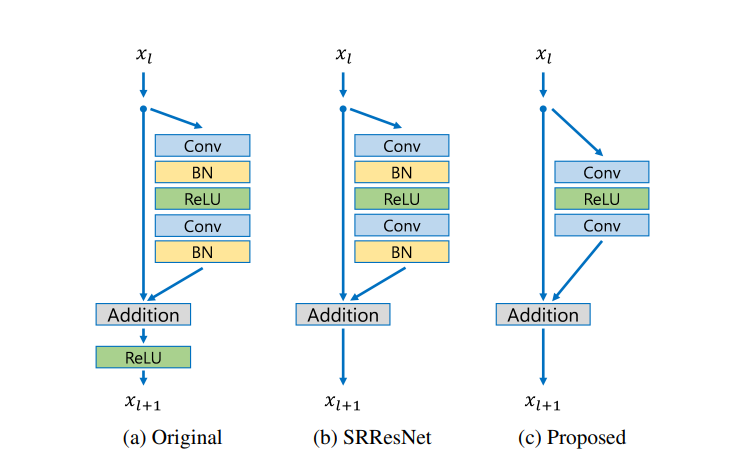
\includegraphics[bb = 92 86 545 742, height=6in]{Chapter1/Chapter1Figs/edsr.png}
    \fi
    \caption{ResNet vs SRResNet vs EDSR \cite{lim2017enhanced}}
    \label{EDSR Architecture}
  \end{center}
\end{figure}

The EDSR architecture \cite{lim2017enhanced} is based on the SRResNet architecture. It gives performance better than most state-of-the-art super-resolution models because it doesn't utilize the unnecessary modules present in conventional residual networks, and by increasing the model size.\\


An important feature of the EDSR network is that it can be used for higher magnifications such as 4X and 8X and has been used extensively for various kinds of super-resolution tasks. \\

Despite its large number of training parameters, EDSR is very simple to train and provides a very good PSNR for super-resolution, especially for medical imaging such as MRI which makes it a good baseline model for our work.\ref


\section{W-Net for MRI Reconstruction}

\begin{figure}[!htbp]
  \begin{center}
    \leavevmode
    \ifpdf
      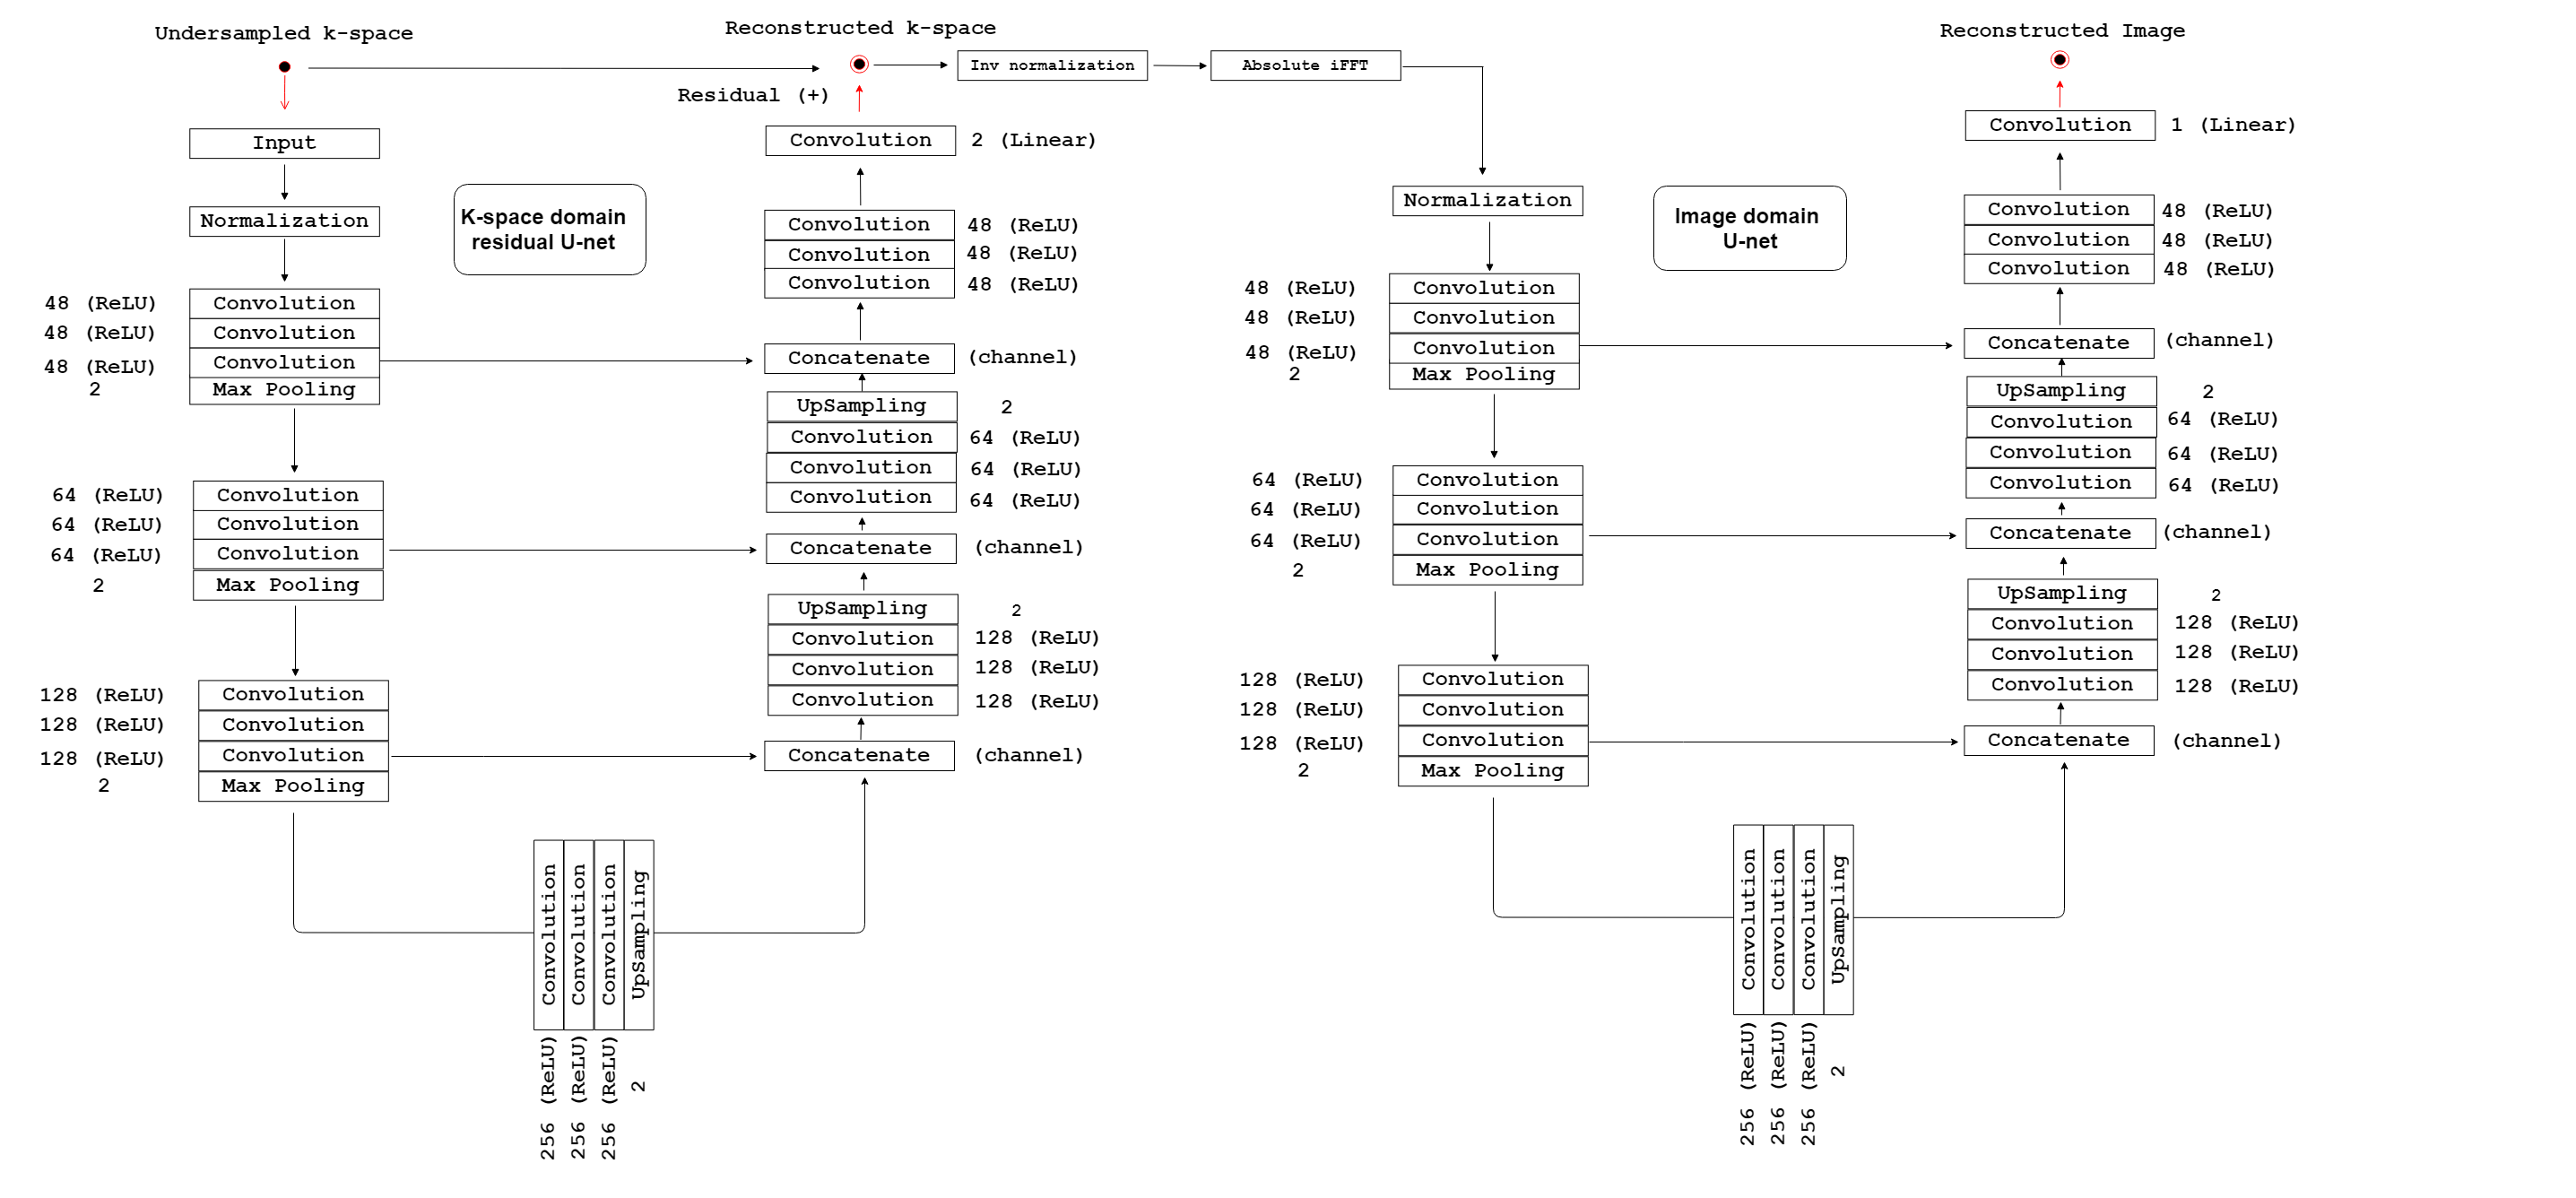
\includegraphics[height=3in]{Chapter1/Chapter1Figs/w-net.png}
    \else
      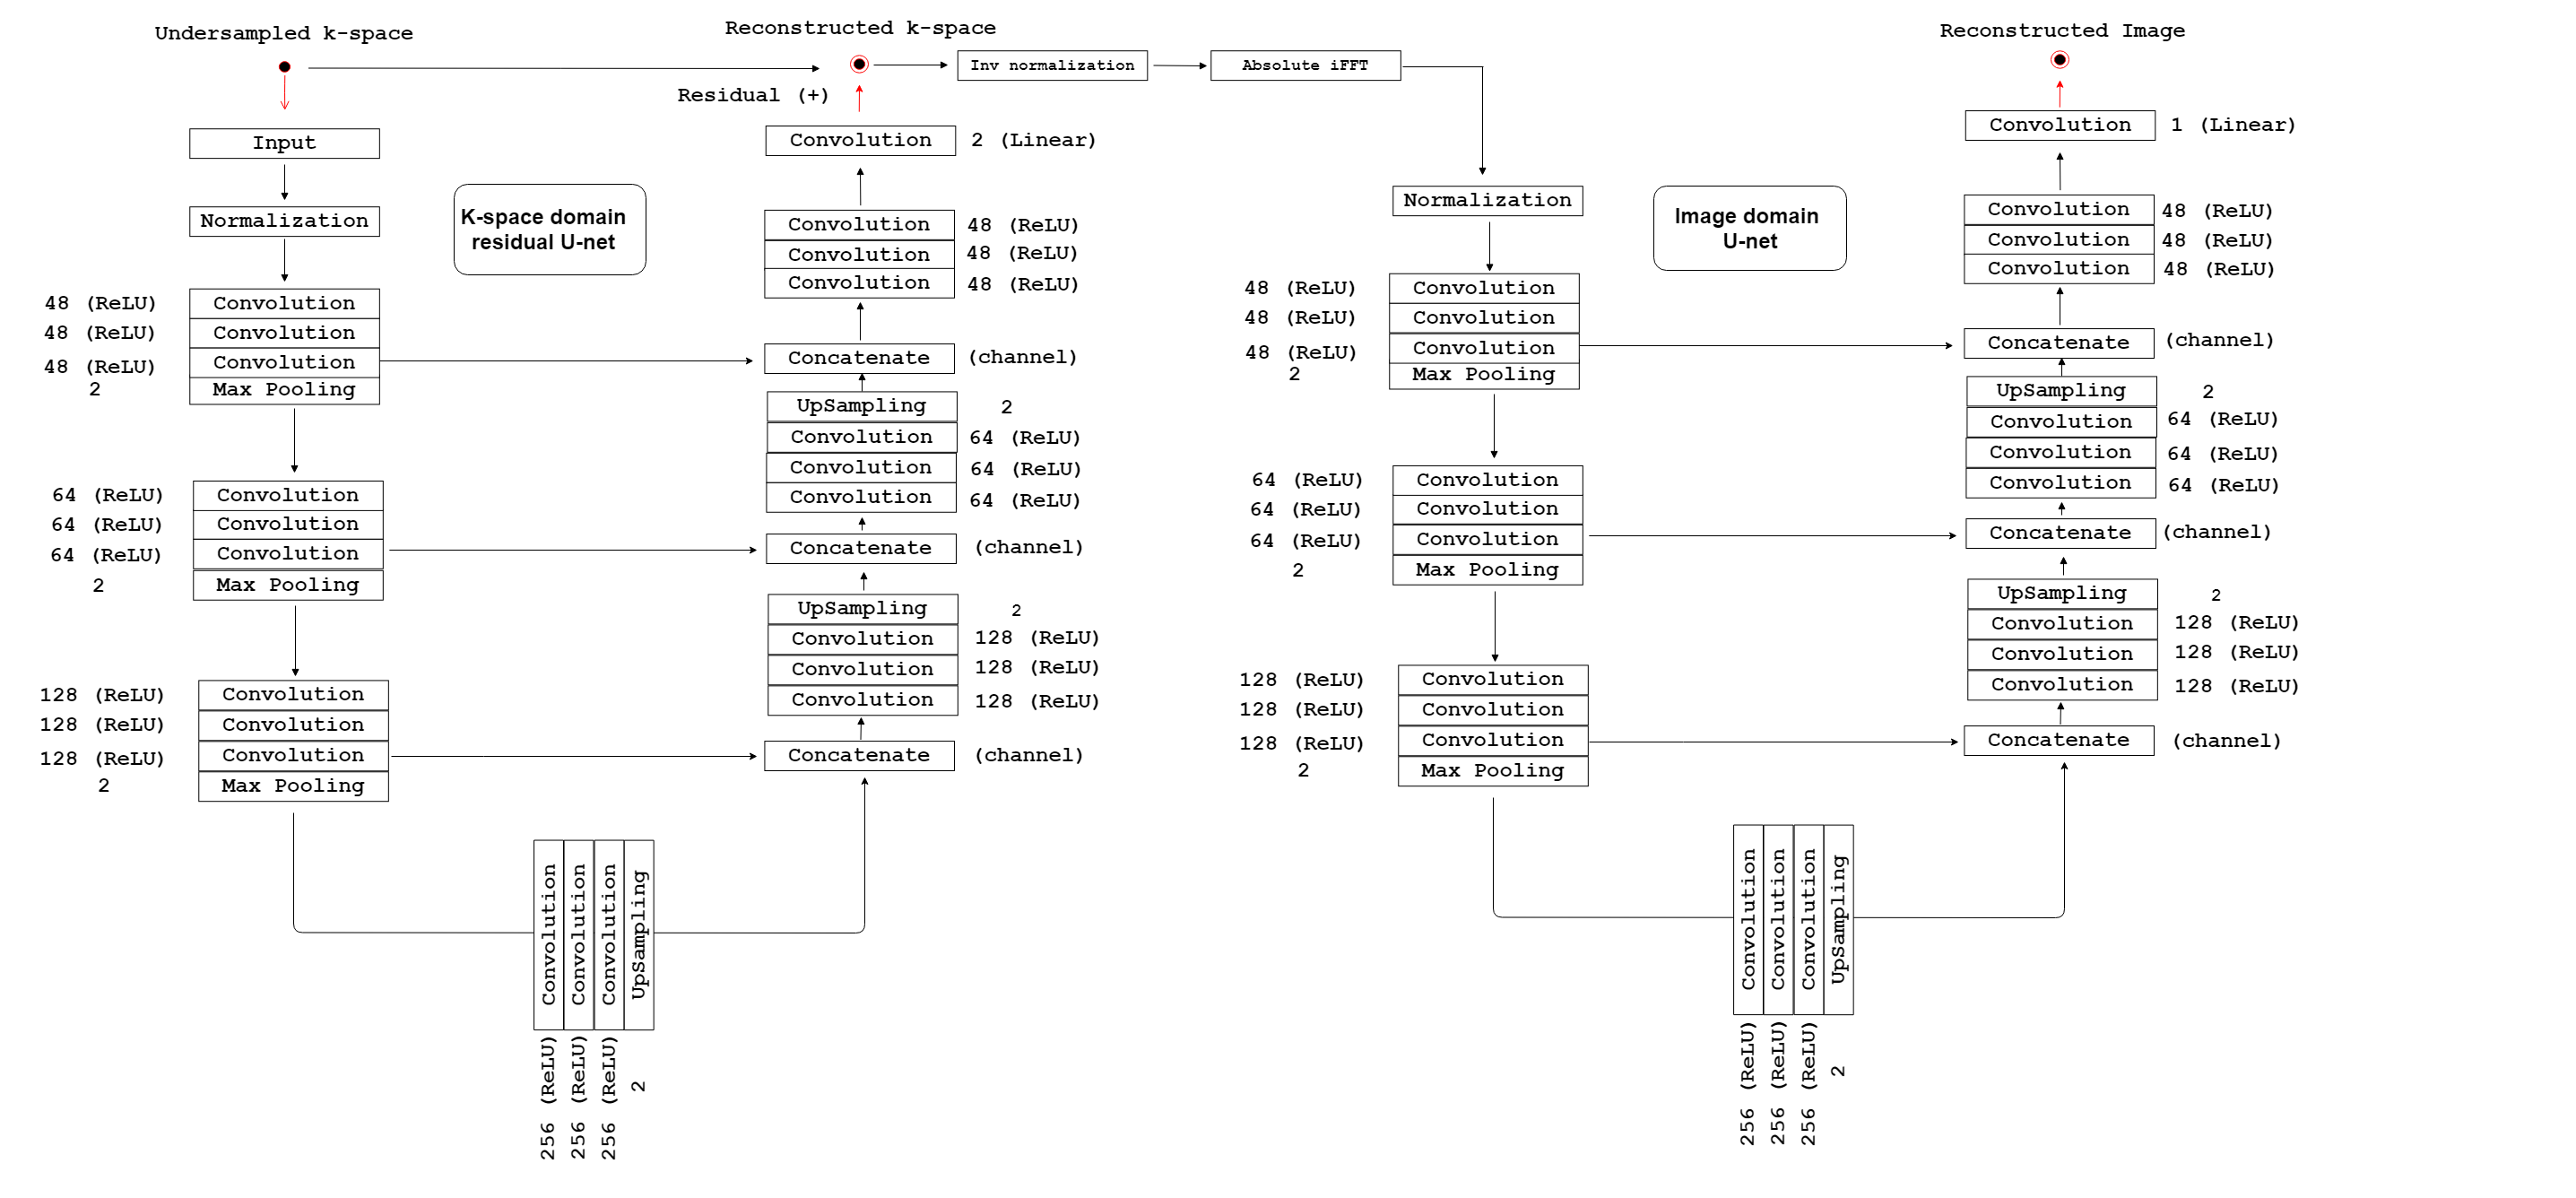
\includegraphics[bb = 92 86 545 742, height=6in]{Chapter1/Chapter1Figs/w-net.png}
    \fi
    \caption{W-Net architecture using two U-Nets \cite{8919674}}
    \label{W-Net model}
  \end{center}
\end{figure}

W-Net is an architecture that comprises two similar U-Nets and works both in the k-space (or frequency-domain) and the image (or spatial) domains. The model uses a complex-valued residual U-Net in the k-space domain, an iFFT operation, and a real-valued U-Net in the image domain (\cite{8919674}). This model is particularly suited to MR Images where there is an availability of raw k-space data to work with before it is converted into the image domain. The overall architecture can be seen in figure \ref{W-Net model} borrowed from \cite{xia2017wnet}.\\



This architecture displayed excellent results for reconstructing MR Images while utilizing lesser resources than other models such as GANs and Deep-Cascade networks. We aim to further enhance this model and tailor it further for MR Images.


\section{Super-Resolution via Repeated Refinements (SR3)}
\nomenclature[zSR3]{$SR3$}{Super-Resolution via Repeated Refinements}

Super-Resolution via Repeated Refinements (SR3) is a super-resolution diffusion model. Diffusion models have sprung up in recent years (\cite{saharia2021image}) as a model that provides accurate results, even more so than the popular Generative-Adversarial Networks (GANs \cite{goodfellow2014generative}) while being easier to train (\cite{dhariwal2021diffusion}).\\

Diffusion models have found their way into medical imaging and have become a popular option for the Super-Resolution of medical images. The SR3 model is trained by taking an image and adding noise to it progressively until only pure noise remains. The model learns to reverse this process so that it can create a high-resolution image from pure noise, iteratively, with guidance from the low-resolution image. Figure \ref{SR3-face} shows how SR3 works by removing noise to produce a high-resolution image, given the low-resolution image for reference (taken from \underline{\href{https://github.com/Janspiry/Image-Super-Resolution-via-Iterative-Refinement}{Janspiry's GitHub page}}).\\




Some popular implementations already exist and use well-known loss functions such as L1 and L2 for training to provide good results. This model showed very promising results, and due to it being a relatively very new model, it is under-researched. We aim to use this model for the super-resolution of MRIs.

\begin{figure}[!htbp]
  \begin{center}
    \leavevmode
    \ifpdf
      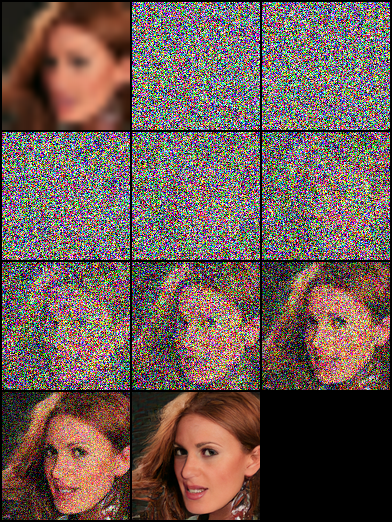
\includegraphics[height=4in]{Chapter1/Chapter1Figs/sr3.png}
    \else
      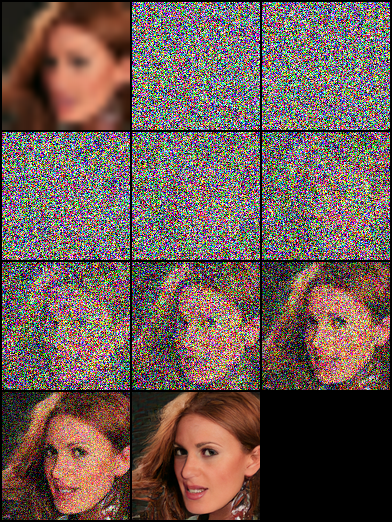
\includegraphics[bb = 92 86 545 742, height=6in]{Chapter1/Chapter1Figs/sr3.png}
    \fi
    \caption{Super-Resolution via Repeated Refinements on a face taken from \href{https://github.com/Janspiry/Image-Super-Resolution-via-Iterative-Refinement}{Janspiry's GitHub page}}
    \label{SR3-face}
  \end{center}
\end{figure}

% \nomenclature[zcif]{$CIF$}{Cauchy's Integral Formula}                                % first letter Z is for Acronyms 
% \nomenclature[aF]{$F$}{complex function}                                                   % first letter A is for Roman symbols
% \nomenclature[gp]{$\pi$}{ $\simeq 3.14\ldots$}                                             % first letter G is for Greek Symbols
% \nomenclature[gi]{$\iota$}{unit imaginary number $\sqrt{-1}$}                      % first letter G is for Greek Symbols
% \nomenclature[gg]{$\gamma$}{a simply closed curve on a complex plane}  % first letter G is for Greek Symbols
% \nomenclature[xi]{$\oint_\gamma$}{integration around a curve $\gamma$} % first letter X is for Other Symbols
% \nomenclature[rj]{$j$}{superscript index}                                                       % first letter R is for superscripts
% \nomenclature[s0]{$0$}{subscript index}                                                        % first letter S is for subscripts

% \section{Second Paragraph}
% and here I write more ...\cite{texbook}

% \subsection{sub first paragraph}
% ... and some more ...

% Now I would like to cite the following: \cite{latex} and \cite{texbook}
% and \cite{Rud73}.

% I would also like to include a picture ...

% \begin{figure}[!htbp]
%   \begin{center}
%     \leavevmode
%     \ifpdf
%       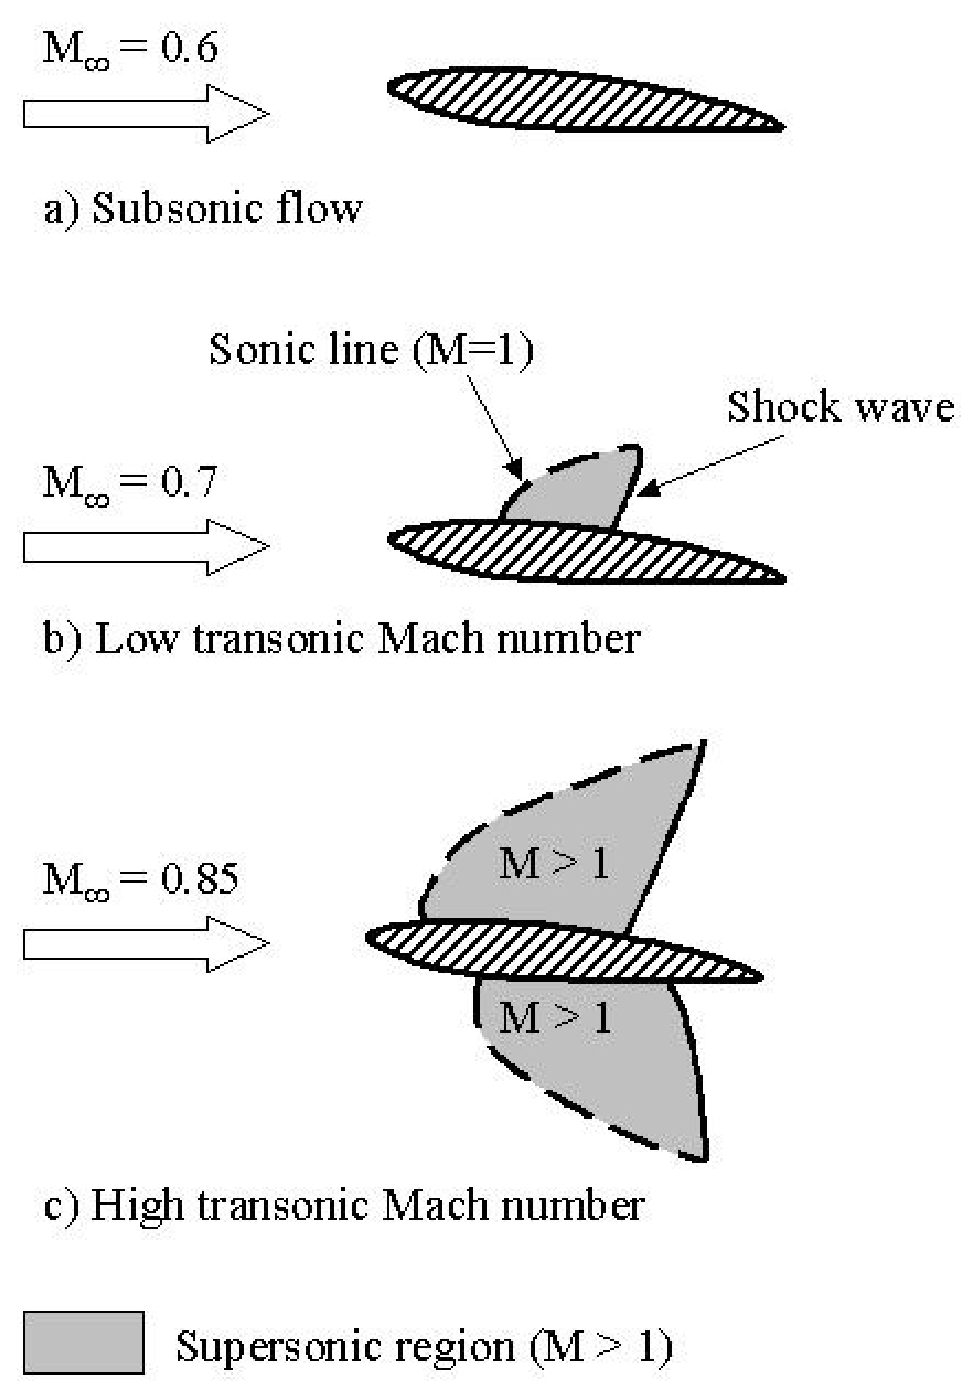
\includegraphics[height=6in]{aflow}
%     \else
%       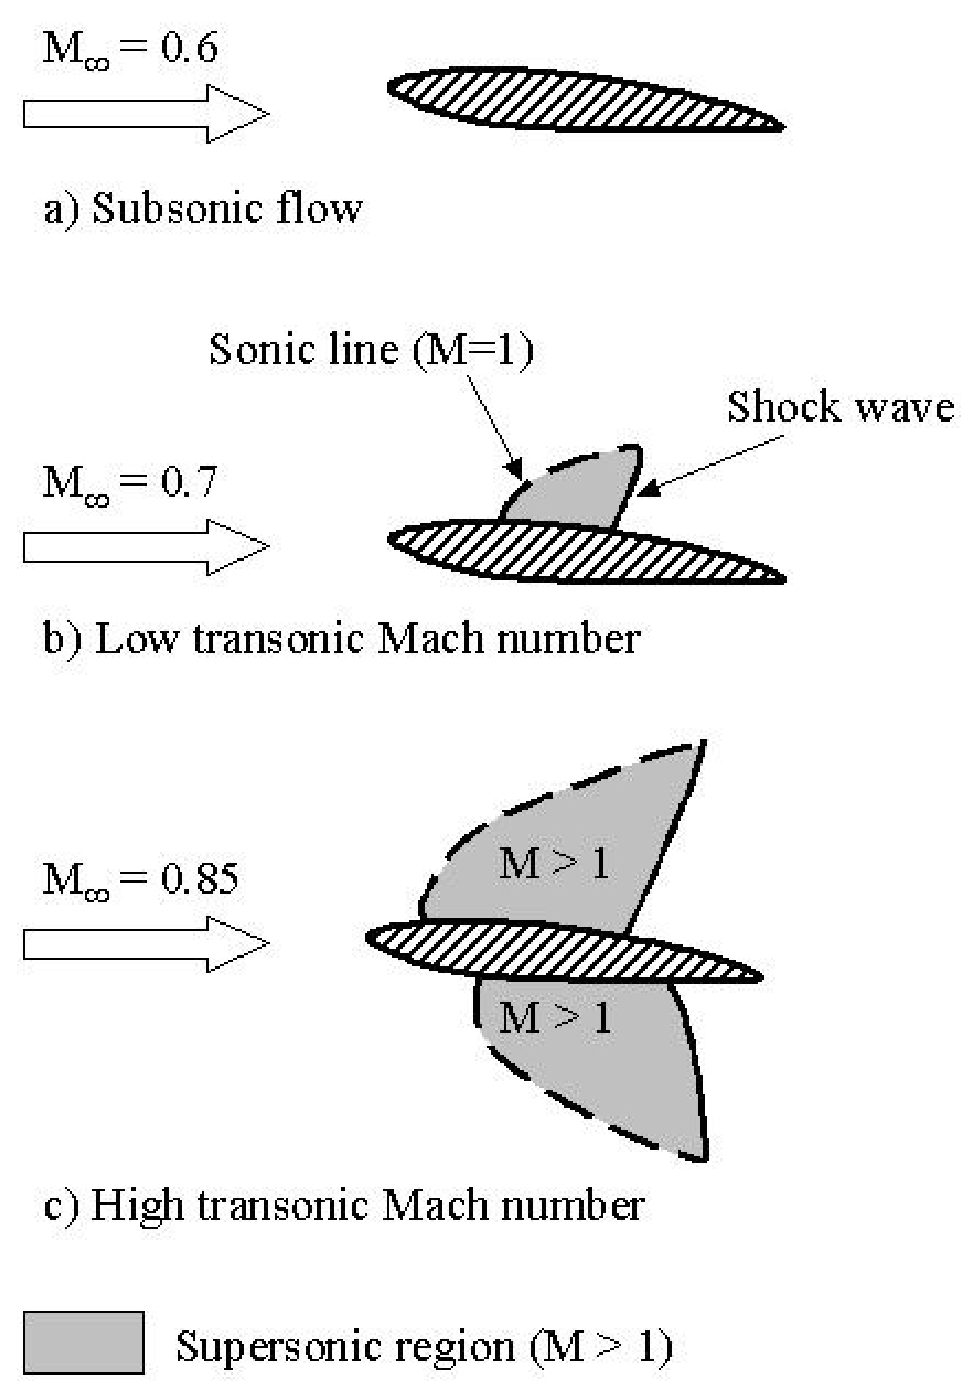
\includegraphics[bb = 92 86 545 742, height=6in]{aflow}
%     \fi
%     \caption{Airfoil Picture}
%     \label{FigAir}
%   \end{center}
% \end{figure}

% % above code has been macro-fied in Classes/MacroFile.tex file
% %\InsertFig{\IncludeGraphicsH{aflow}{6in}{92 86 545 742}}{Airfoil Picture}{FigAir}

% So as we have now labelled it we can reference it, like so (\ref{FigAir}) and it
% is on Page \pageref{FigAir}. And as we can see, it is a very nice picture and we
% can talk about it all we want and when we are tired we can move on to the next
% chapter ...

% I would also like to add an extra bookmark in acroread like so ...
% \ifpdf
%   \pdfbookmark[2]{bookmark text is here}{And this is what I want bookmarked}
% \fi
% ------------------------------------------------------------------------


%%% Local Variables: 
%%% mode: latex
%%% TeX-master: "../thesis"
%%% End: 

\chapter{About the Datasets used}
\ifpdf
    \graphicspath{{Chapter3/Chapter3Figs/PNG/}{Chapter3/Chapter3Figs/PDF/}{Chapter3/Chapter3Figs/}}
\else
    \graphicspath{{Chapter3/Chapter3Figs/EPS/}{Chapter3/Chapter3Figs/}}
\fi

\section{Calgary-Campinas Public MR dataset}\label{sec:3_1}
\markboth{\MakeUppercase{\thechapter. About the Datasets used}}{\thechapter. About the Datasets used}

\nomenclature[zT]{$T$}{Tesla (Measures Magnetic Field Strength)}

A collaborative effort between researchers at the Vascular Imaging Lab located at the University of Calgary and the Medical Image Computing Lab located at the University of Campinas (UNICAMP) resulted in the Calgary-Campinas Public MR dataset \cite{SOUZA2018482}.\\

The Calgary-Campinas Public MR dataset consists of 359 MRIs of healthy adults in the range of 29-80 years old. It consists of images from MRI scanners with two magnetic field strengths 1.5T (Tesla) and 3T (Tesla) and also contains scanners from 3 different companies, they are GE, Philips and Siemens. The data is also well divided among all the six combinations formed by the company name and magnetic field strength with approximately 60 images in each. The dataset is also gender and age-balanced as much as possible with the subjects at hand.\\

\begin{figure}[!htbp]
  \begin{center}
    \leavevmode
    \ifpdf
      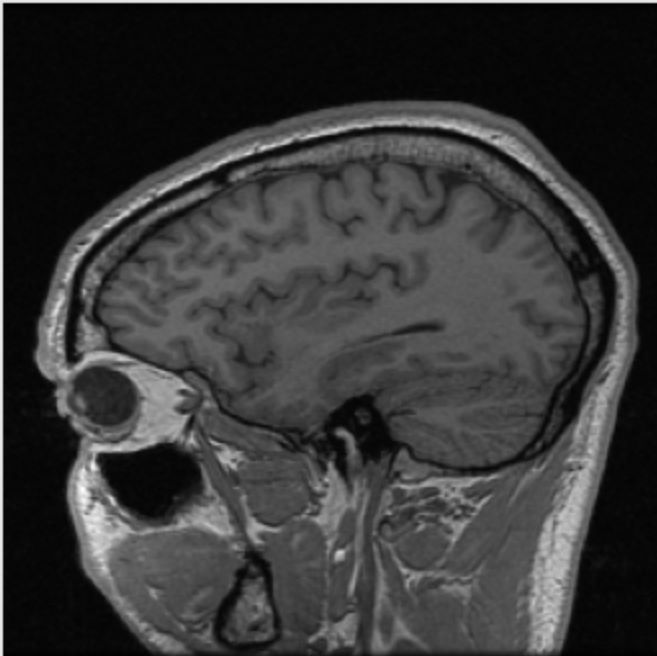
\includegraphics[height=3in]{Chapter3/Chapter3Figs/calgary_campinas_image.jpg}
    \else
      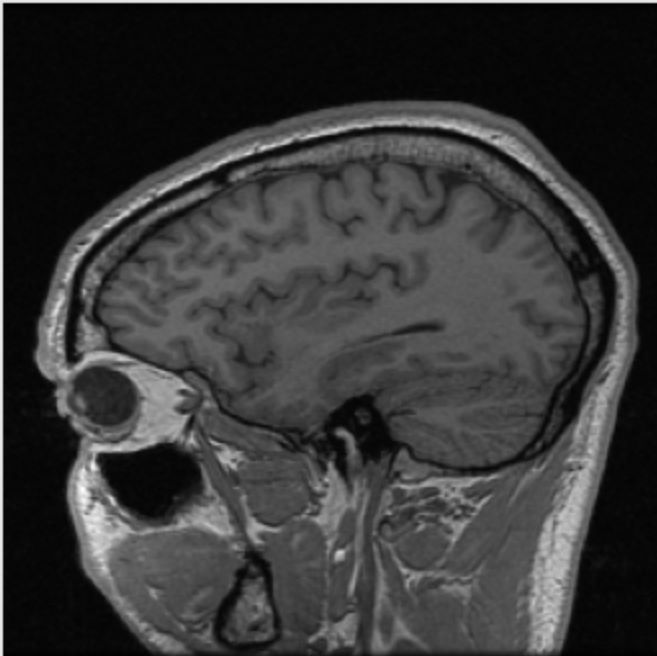
\includegraphics[bb = 92 86 545 742, height=3in]{Chapter3/Chapter3Figs/calgary_campinas_image.jpg}
    \fi
    \caption{Example MRI slice (image domain) from Calgary-Campinas dataset}
    \label{campinas1}
  \end{center}
\end{figure}

We have used 45 sideways brain MRIs from the Calgary-Campinas dataset (Single-channel coil data).\\

The MRIs have been divided into 25 for training (4524 slices), 10 for validation (1700 slices) and 10 for testing (1700 slices). Each MRI has approx 170 slices and the per-slice resolution is 256 X 256.\\

The purpose of using the single coil Calgary-Campinas dataset is to have a dataset that gives sharp images of healthy individuals and also is small enough to easily allow us to work with it, given the limited memory allocated to us on the provided hardware. The dataset was primarily used to train the W-Net, W-Net combined and W-Net 3-layer models, discussed in more detail in \ref{sec:prob_1}.\\

\section{fastMRI dataset}\label{sec:3_2}
\markboth{\MakeUppercase{\thechapter. About the Datasets used }}{\thechapter. About the Datasets used}

The fastMRI dataset \cite{zbontar2019fastmri} is a large-scale collection of both raw MR measurements and clinical MR images, that can be used for training and testing various machine learning approaches including MRI reconstruction, super-resolution, etc.\\

We used a small portion of the brain mulitcoil MRI scan data containing 10-30 slices in each MRI scan and with variable resolutions. We purposed the provided data to give us a fixed resolution of 248 X 248 while ensuring no loss of relevant data and managed to obtain 5473 slices, where 80\% was allotted to training and 20\% was allotted to validation with 50 remaining for training.\\

We used this data initially to train known models such as ESPCN and EDSR to study the existing SR (Super Resolution) models and have a perspective of their capabilities when working with MRIs and the problems that often appear with them.\\

\begin{figure}[!htbp]
  \begin{center}
    \leavevmode
    \ifpdf
      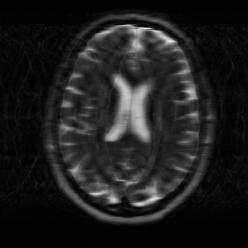
\includegraphics[height=3in]{Chapter3/Chapter3Figs/challenge_brain_Philips_6751018450_AXT2TSE_3_.png}
    \else
      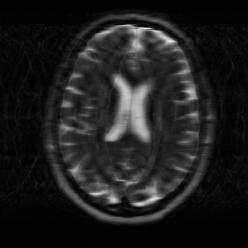
\includegraphics[bb = 92 86 545 742, height=3in]{Chapter3/Chapter3Figs/challenge_brain_Philips_6751018450_AXT2TSE_3_.png}
    \fi
    \caption{An example MRI used from the fastMRI dataset}
    \label{FigFmri}
  \end{center}
\end{figure}

\section{Brain Tumor Segmentation(BraTS2020) dataset}\label{sec:3_3}
\markboth{\MakeUppercase{\thechapter. About the Datasets used }}{\thechapter. About the Datasets used}

The Brain Tumor Segmentation(BraTS2020) dataset \cite{menze2015multimodal, bakas2017advancing, bakas2018identifying} includes pre-operative MRI scans of patients with various types of brain tumours and is often used for brain tumour segmentation and analysis.\\

One MRI scan in the dataset has four different MRI modalities, they are native (T1) scans, post-contrast T1-weighted, T2-weighted and T2-flair. These scans were sourced from many scanners from 19 institutions.\\

The dataset has been purposed to provide us with 3312 images of 512 X 512 MR images. Brain MRI data is preferred for comparison as compared to other regions because of the very fine details present in the brain MRIs along with minimal artefacts that come in especially handy when it comes to Super Resolution tasks.\\

We preferred this dataset over fMRI dataset \ref{sec:3_1} because we observed a ringing effect in the fMRI multicoil scans and hence didn't want to compromise the results of super-resolution because of those artefacts. Calgary-Campinas dataset \ref{sec:3_2} on the other hand works with healthy humans but instead we want the SR problem to focus on a real-world environment. The BraTS dataset provides us with brain tumour MRIs to ensure that the results we obtain are reproducible in a real-world environment for this specific problem. This is because SR is extremely sensitive to varied environments and hence we preferred this dataset for the SR problem.

\begin{figure}[!htbp]
  \begin{center}
    \leavevmode
    \ifpdf
      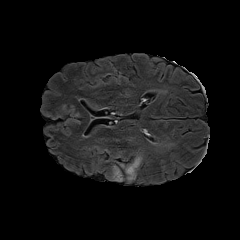
\includegraphics[height=3in]{Chapter3/Chapter3Figs/volume_12_slice_80.png}
    \else
      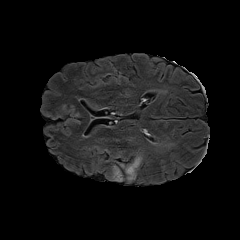
\includegraphics[bb = 92 86 545 742, height=3in]{Chapter3/Chapter3Figs/volume_12_slice_80.png}
    \fi
    \caption{An example MRI used from the BraTS 2020 dataset}
    \label{FigFmri}
  \end{center}
\end{figure}

% ------------------------------------------------------------------------


%%% Local Variables: 
%%% mode: latex
%%% TeX-master: "../thesis"
%%% End: 


\chapter{Our Solutions}\label{ch:soln}
\ifpdf
    \graphicspath{{Chapter2/Chapter2Figs/PNG/}{Chapter2/Chapter2Figs/PDF/}{Chapter2/Chapter2Figs/}}
\else
    \graphicspath{{Chapter2/Chapter2Figs/EPS/}{Chapter2/Chapter2Figs/}}
\fi

\section{MR Reconstruction Problem}\label{sec:prob_1}
\markboth{\MakeUppercase{\thechapter. Our Solutions }}

MR Reconstruction problem is a key area of research where the objective is to speed up the process of taking an MRI, the long wait time is problematic for a large group of patients such as children, people with fear of enclosed spaces, etc. A way to effectively tackle this problem is to take under-sampled MRI scans from a patient and try to fill in the gaps left behind by an incomplete scan with the help of neural networks.\\

Our Solution builds upon the pre-existing W-Net \cite{8919674}. The working of the W-Net architecture goes as follows, it accepts a single k-space slice of an MRI. There are two components of the W-Net -- the first U-Net working in the k-space domain and the other U-Net working in the image domain connected to the output of the previous U-Net (before the information is passed over to the other it is converted back to the image domain). This process works together using a combined loss function, i.e., NRMSE (Normalized Root Mean Square) and gives a certain weightage to each loss (1\% weightage to the U-Net in the k-space domain and 99\% weightage to the U-Net in image domain). The priority here lies in reducing image domain loss.\\

\subsection{Solution to reduce training time ($W-Net$ $Combined$)}

Having limited resources and time is a common problem for medical imaging and we tried to think of a simple way to reduce training time for the model by coming up with the idea to split the W-Net back into two U-Nets and train them independently on two separate machines and then train the two independently trained models together.\\

Individual U-Nets converge in lesser time than the complete W-Net and the idea was that combined training will help the model to converge quicker.\\

The combined network will give results similar to W-Net and train quicker than W-Net.\\

\subsection{Solution to improve image quality ($W-Net\;3-Layer$)}

Having discussed a method to reduce training time, we propose a method to improve on the idea of the W-Net.\\

Our solution uses the pre-existing W-Net architecture \cite{8919674} and adds another component to it, i.e., to use the localised information of the neighbouring slices to help learn the fully sampled MRI reconstruction. Here, instead of feeding one single slice of the MRI to our W-Net, we feed it 3 consecutive slices of an MRI (3 consecutive slices of an MRI are very similar in structure and look, and the information from the nearby slices act as additional information helpful to reconstruct a fully sampled MRI scan slice).\\

We limit our solution to only 3 slices because otherwise the model becomes too large to train given the resources available to us and while it is possible to adjust this parameter to obtain better results, it can be a point to be explored in detail separately.\\

\section{MR Super Resolution Problem}\label{sec:prob_2}
\markboth{\MakeUppercase{\thechapter. My Second Chapter }}

Super Resolution is a well-known problem in deep learning and it has numerous applications in medical imaging as well.\\

Super Resolution of MRIs is a problem for multiple reasons given below.

\begin{enumerate}
\item MR images are more prone to noise because of reasons such as the motion of the patient, and noise caused by nearby electronics.

\item Large amount of data is required for training a super-resolution model but it's difficult to come by a large amount of medical imaging data.

\item MRIs contain complex features such as tissue contrast, noise, etc. that make it difficult to predict the high-resolution from the low-resolution image.
\end{enumerate}

Our goal is to tackle the main bottleneck that appears in medical imaging and that is the requirement of a large dataset size. To tackle this issue we used a pre-trained SR3 model, this pre-trained model had already been trained on human face data and performed well in SR tasks in reference to human faces.\\

The issue of SR quality in MR images is another concern that we tackle by changing the likeness criterion for judging images. It's popular to use criteria such as L1 and L2 loss; they work well enough in general cases. But for MRIs, it's essential to capture the subtle details and show a contrast between different structures.\\

To achieve the above, we propose the use of judgement criteria such as the use of SSIM (Structural Similarity Index) \cite{1284395} and FID (Fréchet Inception Distance) \cite{fid}. While FID and SSIM work well in terms of promoting structural similarity between the SR and the HR MR image, it causes noise to creep in and doesn't work as well as L1 or L2 loss when it comes to reducing the noise in the final resultant image.\\

The idea is to use a mixture of both the structural similarity promoting criterion and the criterion that promotes the reduction of noise, hence a mixture of both is used and we end up with two new approaches that we shall refer to as SSIM Regularized SR3 and FID Regularized SR3.\\

Both of the approaches use a combination of MSE with either SSIM or FID. The objective here is to study the impact of these on the resultant image in comparison to the original SR3.\\

\nomenclature[zsr]{$SR$}{Super Resolution}
\nomenclature[zhr]{$HR$}{High Resolution}

The approaches discussed in this chapter will be discussed in more detail in Chapter \ref{Observations chapter} and there we will also compare the approaches to their original counterparts and present the observations related to them.

% here we don't use MSE (Mean Square Error) as a judgement parameter for the likeness of two images because it doesn't ensure minimisation of artefacts, instead, we propose the use of SSIM (Structural Similarity Index) ~\cite{1284395} and FID (Fréchet Inception Distance) ~\cite{fid}


% ------------------------------------------------------------------------

%%% Local Variables: 
%%% mode: latex
%%% TeX-master: "../thesis"
%%% End: 

\def\baselinestretch{1}
\chapter{Observations} \label{Observations chapter}
\ifpdf
    \graphicspath{{Conclusions/ConclusionsFigs/PNG/}{Conclusions/ConclusionsFigs/PDF/}{Conclusions/ConclusionsFigs/}}
\else
    \graphicspath{{Conclusions/ConclusionsFigs/EPS/}{Conclusions/ConclusionsFigs/}}
\fi

\def\baselinestretch{1.66}

\section{Part 1 -- W-Net}\label{sec:ob_wnet}

We experimented with two different model architectures; W-Net Combined and W-Net 3-layer. We discuss the observations relating to these below, against W-Net\footnote{W-Net comparison model taken from \underline{\href{https://github.com/rmsouza01/Hybrid-CS-Model-MRI}{rmsouza01's GitHub page}}}. The input was corrupted in the k-space domain for training and testing using a random 80\% undersampling mask (example in fig \ref{k-space mask}) to retain only 20\% of the k-space data.


\begin{figure}[!htbp]
  \begin{center}
    \leavevmode
    \ifpdf
      
\includegraphics[height=1.5in]{Chapter4/images/k-space-mask.png}
    \else
      
\includegraphics[bb = 92 86 545 742, height=3in]{Chapter4/images/k-space-mask.png}
    \fi
    \caption{80 \% undersampling mask for k-space}
    \label{k-space mask}
  \end{center}
\end{figure}



\vspace*{0.3cm}
\begin{table}[h]
\begin{center}
\begin{tabular}{ p{4cm} m{3cm} m{3cm} m{3cm} }
 \hline
 \multicolumn{4}{c}{Comparison table -- W-Net models} \\
 \hline
 & PSNR & SSIM & Parameters \\
 \hline
 \hline
 \textbf{W-Net}    & $33.24 \pm 2.92$ & 0.8829 & 4M\\
 \hline
 \textbf{W-Net Combined}& $31.22 \pm 3.28 $& 0.7832 & 2+2+4 M\\
 \textbf{W-Net 3-layer}& $32.21 \pm 0.53$  & 0.8385 & 4M\\
 \hline
\end{tabular}
\end{center}
\caption{Comparison between W-Net models}
\label{W-Net table}
\end{table}

\subsection{W-Net Combined}


\vspace*{0.5cm}
\begin{figure}[!htbp]
  \begin{center}
    \leavevmode
    \ifpdf
      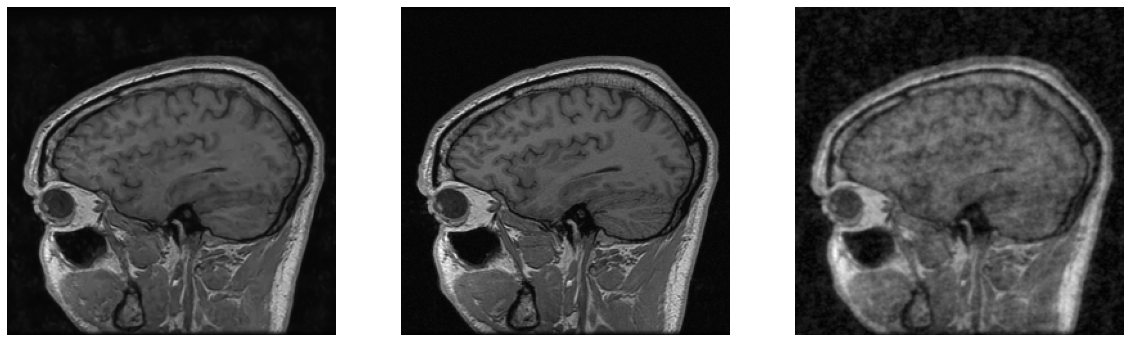
\includegraphics[height=1.5in]{Chapter4/images/res1.png}
    \else
      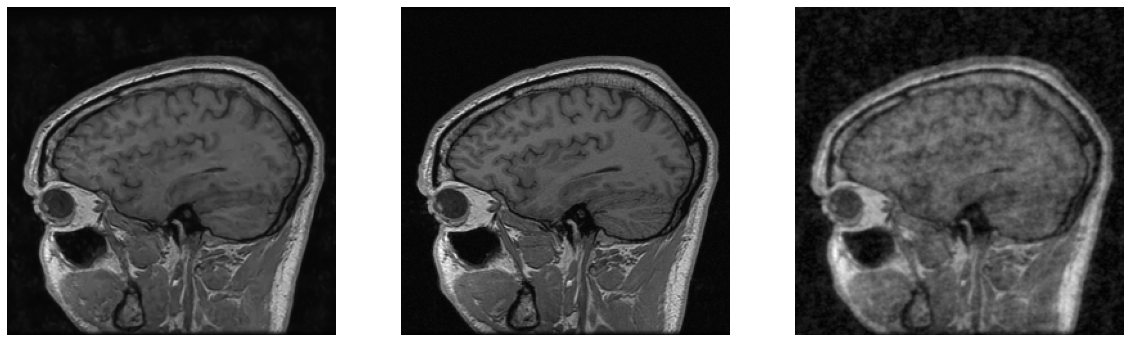
\includegraphics[bb = 92 86 545 742, height=3in]{Chapter4/images/res1.png}
    \fi
    % \caption{Result 1 }
    % \label{Result 1 W-Net Combined}
  \end{center}

  \begin{center}
    \leavevmode
    \ifpdf
      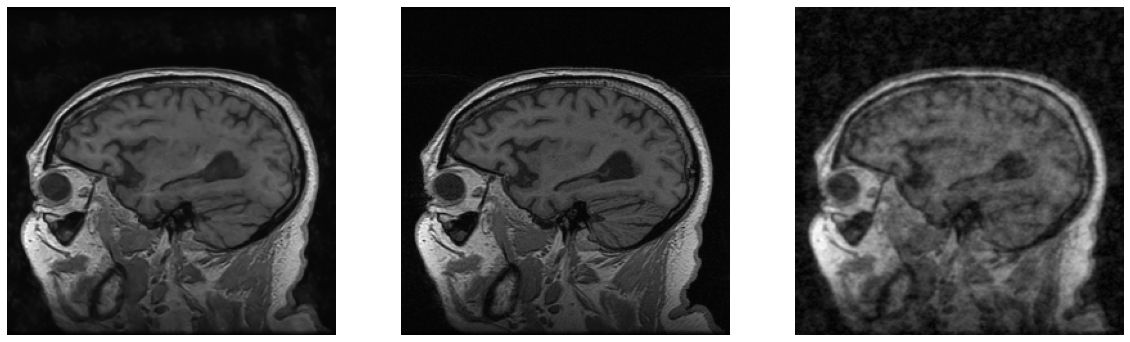
\includegraphics[height=1.5in]{Chapter4/images/res2.png}
    \else
      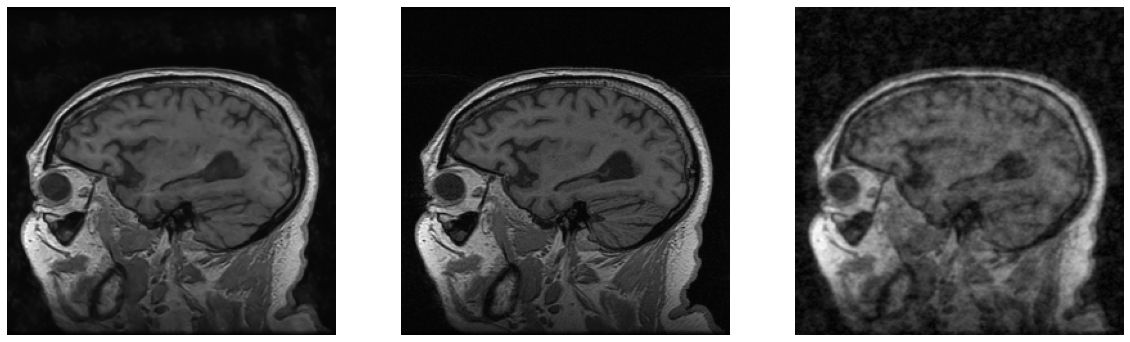
\includegraphics[bb = 92 86 545 742, height=3in]{Chapter4/images/res2.png}
    \fi
    \caption{W-Net Combined results -- Predicted (Left), Original (Middle), Undersampled (Right)}
    \label{Result W-Net Combined}
  \end{center}
\end{figure}

We trained Part 1 (k-space domain) and Part 2 (image domain) of the models separately for 20 epochs each on the k-space data for 25 MRIs, with 10 for validation, and finally trained the whole combined model by joining the two previously trained parts for 15 epochs. Each MRI contained around 170 image slices. The training was done on a Tesla T4 GPU.\\

We don't have comparisons to other super-resolution algorithms such as EDSR or Bicubic interpolation because the image was corrupted in the k-space domain and retains the same pixel dimensions as the original. This is MR reconstruction rather than super-resolution.\\

We can see from figure \ref{Result W-Net Combined} that a lot of the fine details are visible in the prediction and is very true to the original. The PSNR is very close (table \ref{W-Net table}) to the original W-Net, all while using significantly lesser computational time because of the split training technique. We believe that this model is an improvement over the original W-Net as it gives comparable results while reducing the training time and hardware requirements.


\subsection{W-Net 3-layer}

\vspace*{0.5cm}
\begin{figure}[!htbp]
  \begin{center}
    \leavevmode
    \ifpdf
      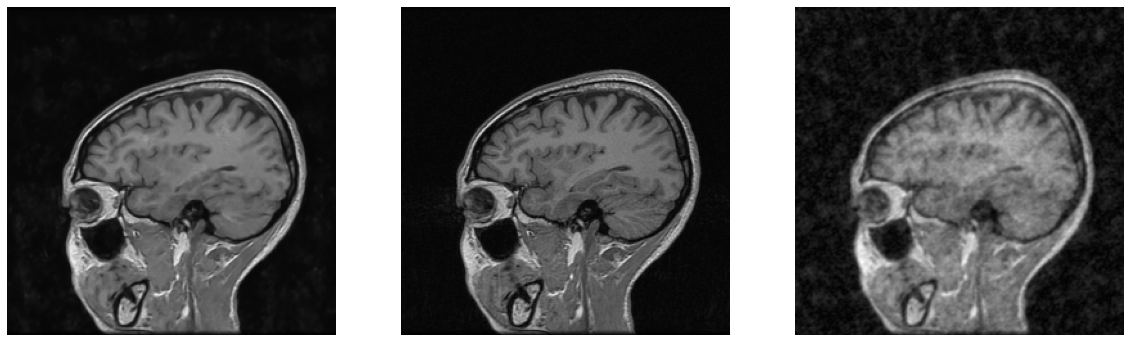
\includegraphics[height=1.5in]{Chapter4/images/res3.png}
    \else
      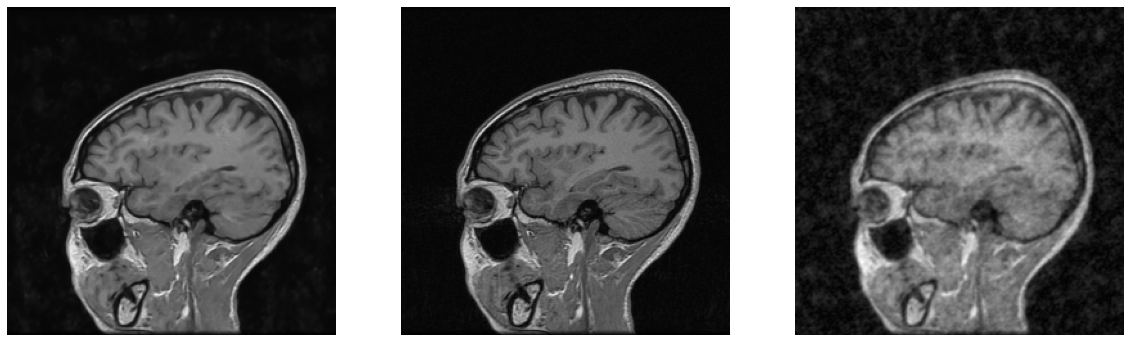
\includegraphics[bb = 92 86 545 742, height=3in]{Chapter4/images/res3.png}
    \fi
    % \caption{Result 1 }
    % \label{Result 1 W-Net Combined}
  \end{center}

  \begin{center}
    \leavevmode
    \ifpdf
      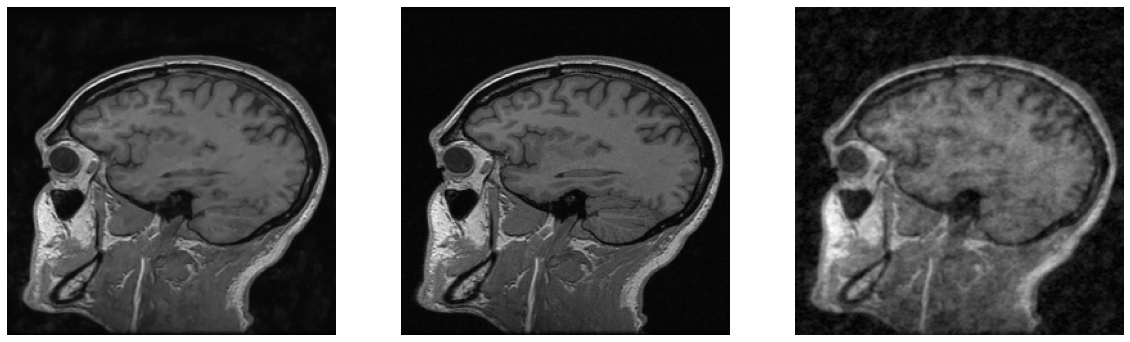
\includegraphics[height=1.5in]{Chapter4/images/res4.png}
    \else
      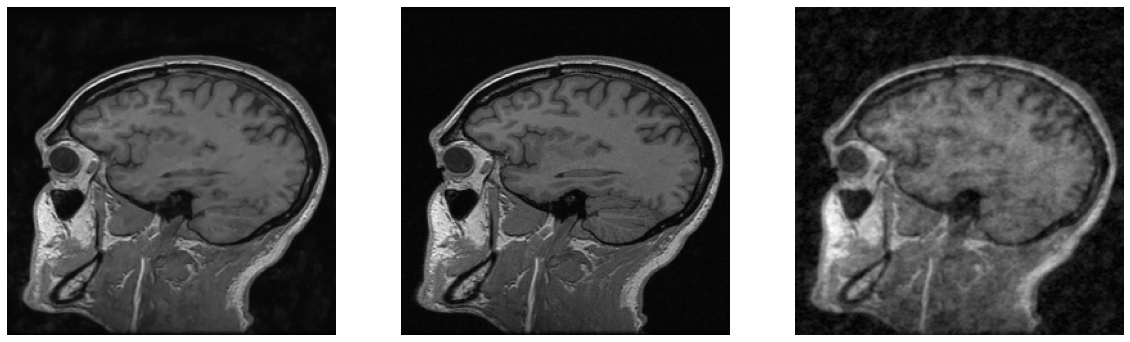
\includegraphics[bb = 92 86 545 742, height=3in]{Chapter4/images/res4.png}
    \fi
    \caption{W-Net 3-layer results -- Predicted (Left), Original (Middle), Undersampled (Right)}
    \label{Result W-Net 3-layer}
  \end{center}
\end{figure}

We trained the model for 25 MRIs and validated it with 10 MRIs. Each MRI has about 170 slices so there are 170-(3-1)=168 inputs (3 slices combine to form one input). Training was done on a Tesla T4 GPU for 30 epochs.\\

As evident from figure \ref{Result W-Net 3-layer} and table \ref{W-Net table}, the model performed on par with the original W-Net and was able to reproduce the fine details such as the folds in the cerebellum, despite the much lesser number of parameters (to fit with the limitations of current hardware) and less number of epochs (75 vs 30). If given better hardware and more time, this model will definitely be able to outperform the original W-Net on the given dataset. This model has a lot of potential and needs to be explored further using better hardware to get exceptional results.


\section{SR3 - Diffusion Model} \label{Observation - SR3}

The SR3 model was trained over a number of different loss functions to improve image super-resolution quality.
\begin{enumerate}
    \item L2 loss
    \item FID
    \item SSIM
    \item FIDR - FID regularized (75\% normalized PSNR, 25\% normalized FID)
    \item SSIMR - SSIM regularized (75\% normalized PSNR, 25\% SSIM)
\end{enumerate}

The following are the results --\\


\begin{table}[h]
\begin{center}
\begin{tabular}{ p{4cm} m{3cm} m{3cm} }
 \hline
 \multicolumn{3}{c}{Comparison table -- SR3} \\
 \hline
 & PSNR & SSIM \\
 \hline
 \hline
 \textbf{Bicubic} & $35.10 \pm 1.22$ & 0.8275\\
 \textbf{L2}    & $34.25 \pm 2.44$ & 0.8233 \\
 \hline
 \textbf{FID}& $35.58 \pm 0.63$  & 0.8354 \\
 \textbf{SSIM}& $36.12 \pm 0.59 $& 0.8618 \\
  \textbf{FIDR}& $36.20 \pm 0.35$  & \textbf{0.8632} \\
 \textbf{SSIMR}& $\bf{36.77 \pm 0.34 }$& 0.8569 \\
 \hline
\end{tabular}
\end{center}
\caption{Comparison between loss functions in SR3}
\label{SR3 table}
\end{table}

FIDR, SSIMR, and Bicubic Interpolation -- all perform at a similar level if seen from the perspective of PSNR (as seen in table \ref{SR3 table}) but PSNR is not able to distinguish well when it comes to scenarios where one image may have distortions or artefacts while another may not and they end up having the same PSNR when compared with the true image.\\

Hence, we will be giving more weightage when it comes to the judgement of quality to SSIM that can capture the perceptual quality of an image in a way that is more similar to humans as compared to PSNR.\\

SSIMR and FIDR models almost perform on a similar level with SSIMR showing the best qualitative results out of all. This shows that having a parameter that gives more weightage to structural similarity performed better as compared to vanilla SR3.\\

The L2 model i.e., the vanilla SR3, and bicubic interpolation showed a decently high PSNR but lagged behind when it came to factors such as structural similarity. Even with the naked eye, one can observe that L2 in Fig. \ref{SR3 L2} wasn't able to give a structurally accurate result when compared to, say, SSIMR in Fig. \ref{Result SR3 - SSIMR}. In the original SR3 paper, they used human subjects and fool rate to get an idea of what image is original when it comes to the judgement of human subjects. Here, we leave the judgement to the reader to observe the difference between the results of these and SSIMR or FIDR.\\

On the other hand, we observed that SSIM and FID seemed to give worse performance than SSIMR of FIDR and also had more noise in their result as compared to the others.\\

Finally, we would like to conclude our observations by saying that the results seem to show that there definitely is a correlation between having a loss function that gives weightage to structural similarity and MRI results that are more structurally similar to the original.

\begin{figure}[!htbp]
  \begin{center}
    \leavevmode
    \ifpdf
      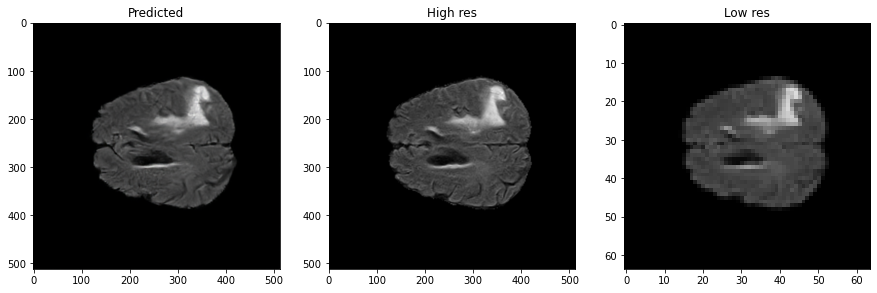
\includegraphics[height=2in]{Chapter4/images/spam1.png}
    \else
      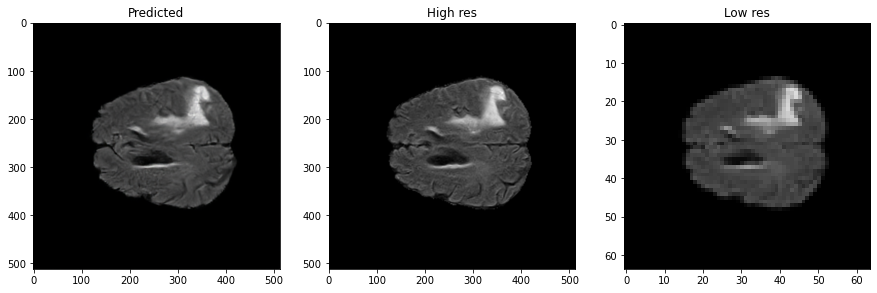
\includegraphics[bb = 92 86 545 742, height=3in]{Chapter4/images/spam1.png}
    \fi
    \caption{SR3 with L2}
    \label{SR3 L2}
  \end{center}
\end{figure} 

\begin{figure}[!htbp]
  \begin{center}
    \leavevmode
    \ifpdf
      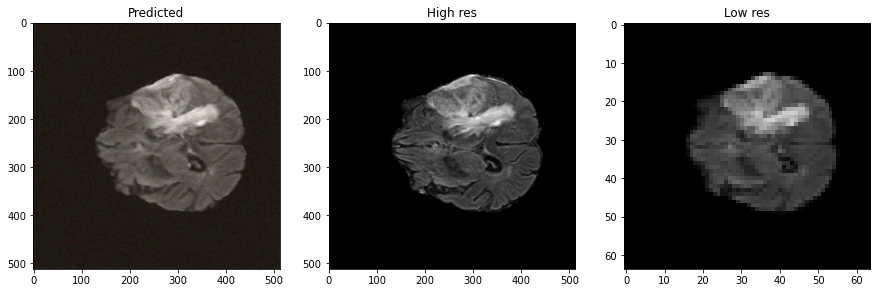
\includegraphics[height=2in]{Chapter4/images/spam3.png}
    \else
      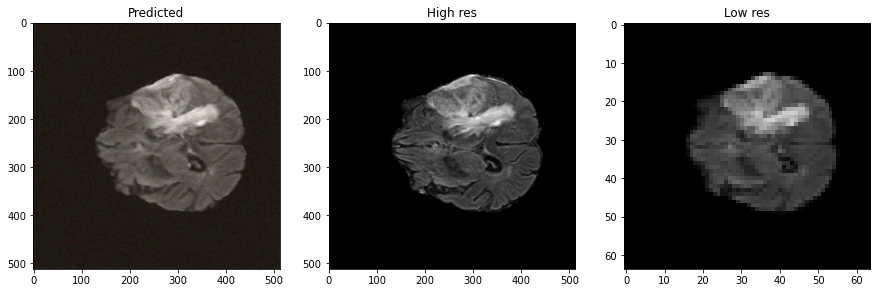
\includegraphics[bb = 92 86 545 742, height=3in]{Chapter4/images/spam3.png}
    \fi
    \caption{SR3 with FID}
    \label{SR3 FID}
  \end{center}
\end{figure} 

\begin{figure}[!htbp]
  \begin{center}
    \leavevmode
    \ifpdf
      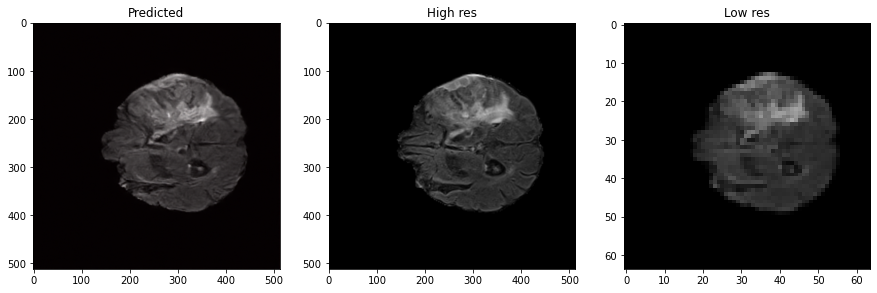
\includegraphics[height=2in]{Chapter4/images/spam2.png}
    \else
      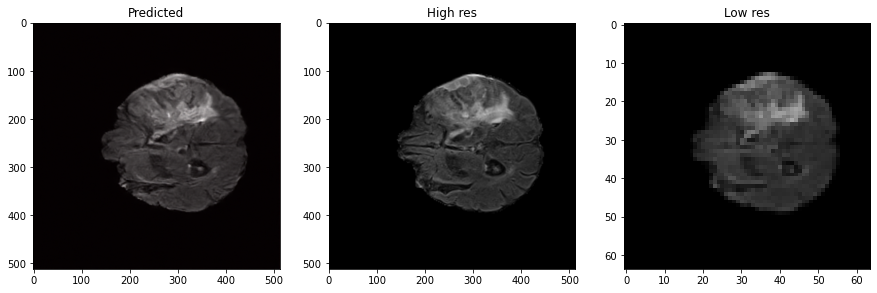
\includegraphics[bb = 92 86 545 742, height=3in]{Chapter4/images/spam2.png}
    \fi
    \caption{SR3 with SSIM}
    \label{SR3 SSIM}
  \end{center}
\end{figure} 



\begin{figure}[!htbp]
  \begin{center}
    \leavevmode
    \ifpdf
      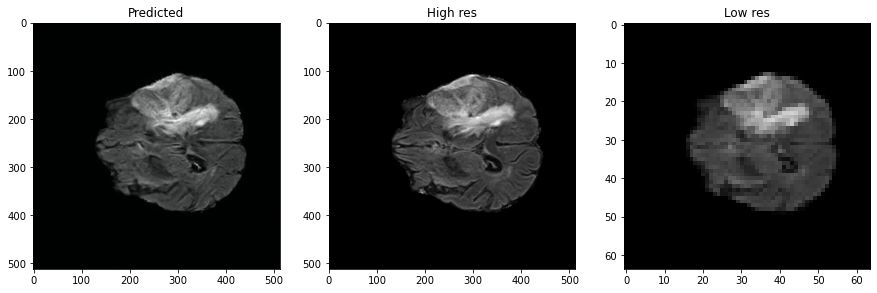
\includegraphics[height=2in]{Chapter4/images/spam4.png}
    \else
      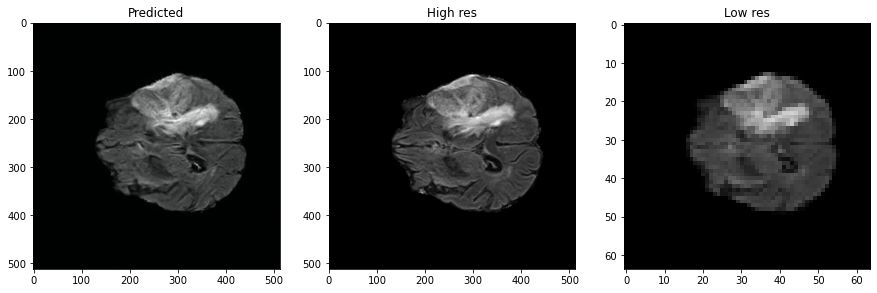
\includegraphics[bb = 92 86 545 742, height=3in]{Chapter4/images/spam4.png}
    \fi
    \caption{SR3 with FIDR}
    \label{SR3 FIDR}
  \end{center}
\end{figure} 


\begin{figure}[!htbp]
  \begin{center}
    \leavevmode
    \ifpdf
      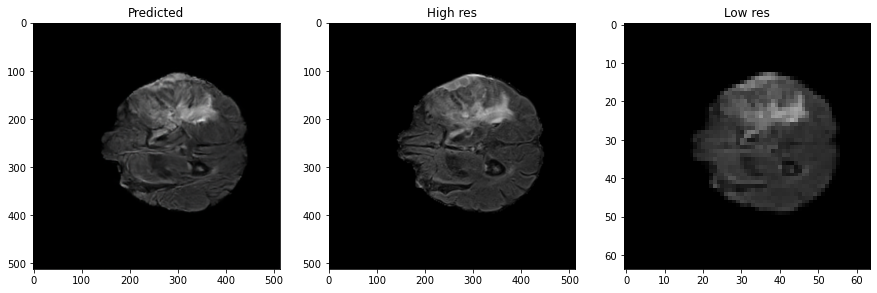
\includegraphics[height=2in]{Chapter4/images/sr3-res1.png}
    \else
      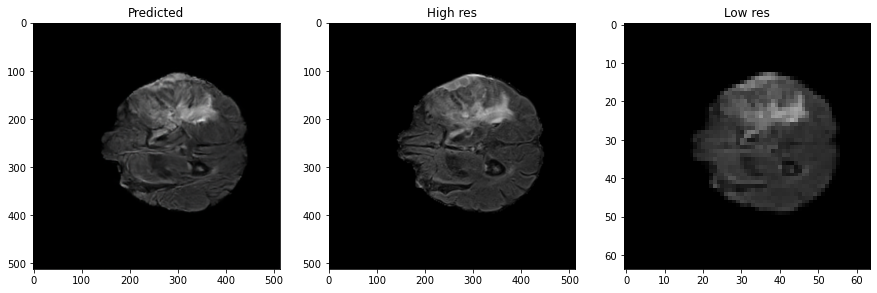
\includegraphics[bb = 92 86 545 742, height=3in]{Chapter4/images/sr3-res1.png}
    \fi
    % \caption{Result 1 }
    % \label{Result 1 W-Net Combined}
  \end{center}

  \begin{center}
    \leavevmode
    \ifpdf
      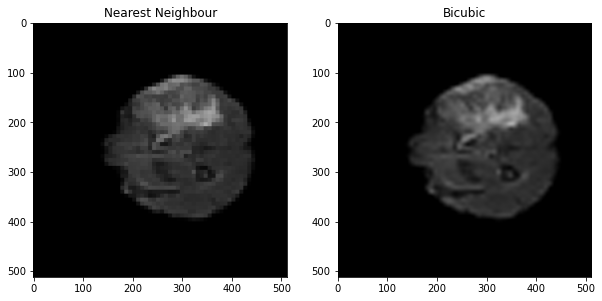
\includegraphics[height=2in]{Chapter4/images/sr3-res2.png}
    \else
      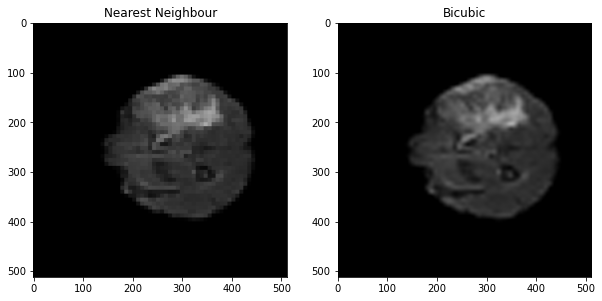
\includegraphics[bb = 92 86 545 742, height=3in]{Chapter4/images/sr3-res2.png}
    \fi
    \caption{SR3 with SSIMR}
    \label{Result SR3 - SSIMR}
  \end{center}
\end{figure}




%%% ----------------------------------------------------------------------

% ------------------------------------------------------------------------

%%% Local Variables: 
%%% mode: latex
%%% TeX-master: "../thesis"
%%% End: 

\def\baselinestretch{1}
\chapter{Conclusion}
\ifpdf
    \graphicspath{{Conclusions/ConclusionsFigs/PNG/}{Conclusions/ConclusionsFigs/PDF/}{Conclusions/ConclusionsFigs/}}
\else
    \graphicspath{{Conclusions/ConclusionsFigs/EPS/}{Conclusions/ConclusionsFigs/}}
\fi

From the observations made earlier, we can conclude the following for each of the solutions discussed in Chapter \ref{ch:soln}.\\

Solution 1 discussed in section \ref{sec:prob_1} talks about the MR reconstruction problem and our solution to the two issues faced in medical imaging were W-Net Combined and W-Net 3-Layer using the pre-existing W-Net Architecture \cite{8919674}.\\

From the observations made about W-Net Combined in \ref{sec:ob_wnet}, it can be seen that the model performed at par with the original W-Net while consuming less time to train than the original W-Net.\\

The observations made about the W-Net 3-Layer show that the model also performed at par with the W-Net but with reduced convolution layers to adjust for the low specs of the hardware allotted to us. Despite the following issue, the model showed great performance with very low variance and showed a promise for improvement if trained in a better environment.\\

Solution 2 discussed in section \ref{sec:prob_2} talks about the MR Super Resolution Problem and our solution aims to tackle the issue of quality in MR images, while also aiming to reduce training time and training dataset by using previously trained models on different problems (such as human face super-resolution). The solution proposed by us is the use of FID and SSIM regularization in SR3 algorithm \cite{saharia2021image}.\\

The qualitative observations made in the section \ref{Observation - SR3} show that the SSIM Regularized SR3 performed the best but the difference is small as far as we could observe for 100K iterations and it is possible that the results may go in another direction if the model is trained for more iterations. It is also important to note that the model has a small batch size that may be the cause of high variations thus affecting the results.\\

Overall, while our experiments were limited by resources and time, we still managed to show that the newly proposed models are able to perform at least at par with the existing models or slightly better. We managed to reduce training time with the help of W-Net Combined, showed promise of improved performance with W-Net 3-layer, and showed improved performance with the help of FIDR and SSIMR in SR3 when compared to their baseline models respectively.\\



\backmatter % book mode only
\appendix
\chapter{Appendix A}
\ifpdf
    \graphicspath{{Appendix1/images/}}
\else
    \graphicspath{{Appendix1/images/}}
\fi

\section{About the SR3 SSIM regularized model}

SR3 algorithm works very similar to the original DDPM paper \cite{ho2020denoising}. The training can be described as follows: \\

\begin{enumerate}
    \item repeat

    \item $(x, y_0)$ $\sim$ $p(x,y)$

    \item $\gamma$ $\sim$ p($\gamma$)

    \item $\epsilon$ $\sim$ \mathcal{N}(0, I)

    \item Take a gradient descent step on:
        
        $$ - (\nabla_{\theta}  NPSNR(f_{\theta}(x, y_{t}, \gamma_{t}), \epsilon) + \lambda * SSIM(f_{\theta}(x, y_{t}, \gamma_{t}), \epsilon))$$

    \item until converged
    
\end{enumerate}

\nomenclature[znpsnr]{$NPSNR$}{Normalized Peak Signal-to-Noise Ratio}
\nomenclature[gn]{$\nabla$}{Gradient of a function}
\nomenclature[gg]{$\gamma$}{The variance schedule}
\nomenclature[s0]{$t$}{timestep t}

The above describes the training process, where a random sample is picked, x is the bicubic interpolated image from the LR image and $y_{0}$ is the HR image, $\gamma_{t}$ is the variance schedule constant and it is assumed to be a constant in the model for a given t.\\

The model is used to obtain the SR image back using a T step refinement process as described below in the original SR3 paper.

\begin{figure}[!htbp]
  \begin{center}
    \leavevmode
    \ifpdf
      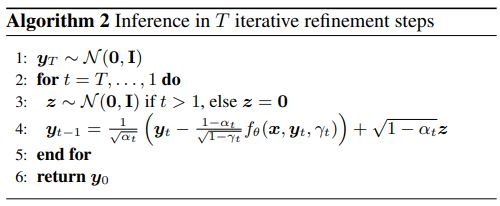
\includegraphics[height=2in]{Appendix1/images/WhatsApp Image 2023-05-08 at 17.34.05.jpg}
    \else
      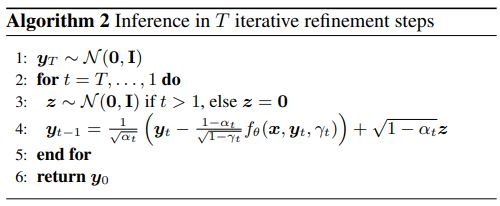
\includegraphics[bb = 50 86 545 742, height=6in]{Appendix1/images/WhatsApp Image 2023-05-08 at 17.34.05.jpg}
    \fi
    \caption{Inference process in T steps using the model learnt in training \cite{saharia2021image}}
    \label{inference_sr3}
  \end{center}
\end{figure}

\begin{figure}[!htbp]
  \begin{center}
    \leavevmode
    \ifpdf
      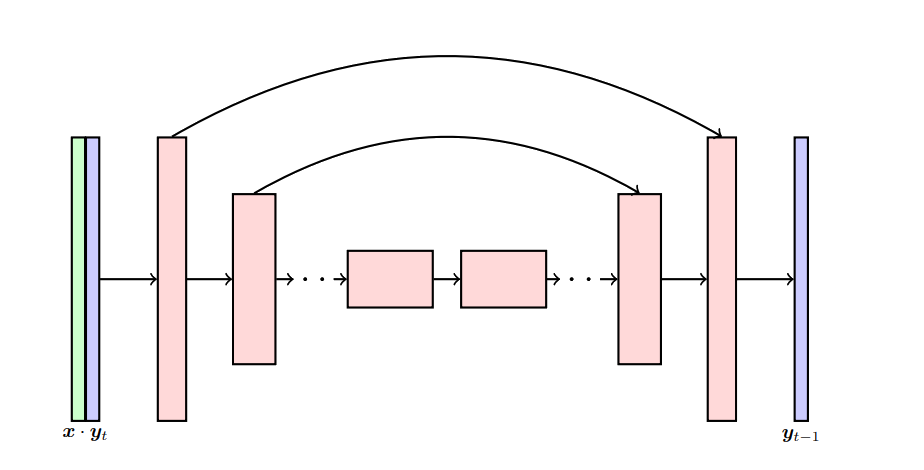
\includegraphics[height=3in]{Appendix1/images/sr3-new.png}
    \else
      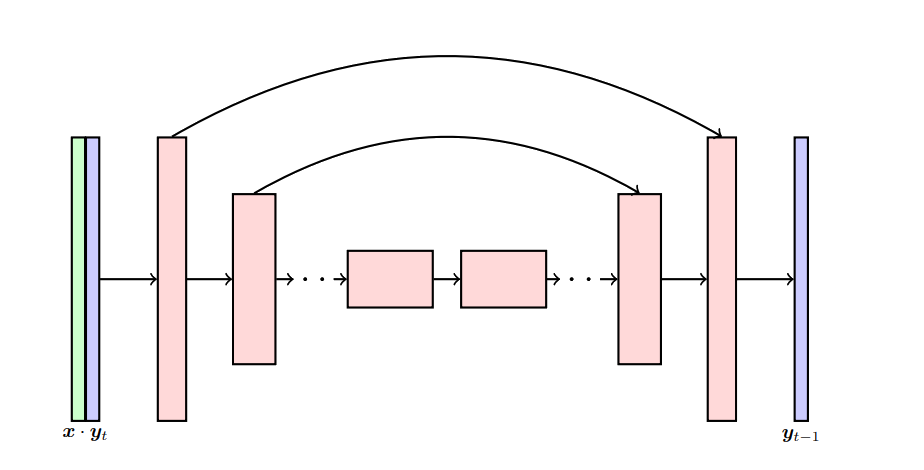
\includegraphics[bb = 92 86 545 742, height=6in]{Appendix1/images/sr3-new.png}
    \fi
    \caption{ Outline of the U-Net showing the input x (the bicubic interpolated image), $y_t$ (the noisy image at timestep t) and the output as $y_{t-1}$ obtained using Algorithm 2 (the noisy image at timestep t-1, less noisy than at timestep t) \cite{saharia2021image}}
    \label{u_net_sr3}
  \end{center}
\end{figure}

\section{Architecture details of our model}

We have trained a variation of the SR3 i.e., SSIM regularized SR3 network with the following details.

\begin{enumerate}
    \item We have focused on the task of converting 64 X 64 MR images to 512 X 512 image datasets.
    \item We have used a pre-trained model (taken from \underline{\href{https://github.com/Janspiry/Image-Super-Resolution-via-Iterative-Refinement}{Janspiry's GitHub page}}), trained on human faces using FFHQ-CelebaHQ dataset \cite{karras2018progressive, karras2019stylebased}.
    \item Other details are included in the table below

    \vspace*{0.3cm}
    \begin{table}[h]
    \begin{center}
    \begin{tabular}{ p{6cm} m{6cm}}
     \hline
     \multicolumn{2}{c}{} \\
     \hline
     \textbf{Channel Multipliers}    & \{1,2,4,8,16\} \\
     \textbf{Timestep T}& 2000\\
     \textbf{Variance Schedule}& Cosine Variance Schedule\\
     \textbf{Batch Size}& 1 (Low GPU memory)\\
     \textbf{Res Blocks}& 1\\
     \textbf{Dropout}& 0\\
     \textbf{Model Parameters}& 155M\\
     \textbf{Train steps}& 100K\\
     \hline
    \end{tabular}
    \end{center}
    \caption{Architecture Details of the Model}
    \label{W-Net table}
    \end{table}
    
\end{enumerate}

The FID model follows the same pattern as SSIM except for the function SSIM being replaced by FID and the architecture details also follow similarly to SSIM. The simple SR3 model also follows the same architecture and parameters but with the absence of regularization.

% ------------------------------------------------------------------------

%%% Local Variables: 
%%% mode: latex
%%% TeX-master: "../thesis"
%%% End: 

% \chapter{Appdx B}

and here I put some more postamble ...

% ------------------------------------------------------------------------

%%% Local Variables: 
%%% mode: latex
%%% TeX-master: "../thesis"
%%% End: 


\bibliographystyle{plainnat}
%\bibliographystyle{Classes/IITRPRbiblio}
\renewcommand{\bibname}{References} % changes default name Bibliography to References
\bibliography{References/references} % References file

\end{document}
